\documentclass[10pt,twocolumn,letterpaper]{article}

\usepackage{cvpr}
\usepackage{times}
\usepackage{epsfig}
\usepackage{graphicx}
\usepackage{amsmath}
\usepackage{amssymb}
\usepackage{float}
\usepackage[english]{babel}
\usepackage{blindtext}
\usepackage{gensymb}
\usepackage{array}
\usepackage{url}
\usepackage{subfigure}
\usepackage{makecell}
%\usepackage[breaklinks=true,bookmarks=false]{hyperref}
\newcolumntype{C}[1]{>{\centering\let\newline\\\arraybackslash\hspace{0pt}}m{#1}}
\newcommand\myworries[1]{\textcolor{red}{#1}}
% Include other packages here, before hyperref.
% Synced in Dropbox
% If you comment hyperref and then uncomment it, you should delete
% egpaper.aux before re-running latex.  (Or just hit 'q' on the first latex
% run, let it finish, and you should be clear).

\cvprfinalcopy % *** Uncomment this line for the final submission

\def\cvprPaperID{****} % *** Enter the CVPR Paper ID here
\def\httilde{\mbox{\tt\raisebox{-.5ex}{\symbol{126}}}}

% Pages are numbered in submission mode, and unnumbered in camera-ready
%\ifcvprfinal\pagestyle{empty}\fi
\setcounter{page}{1}
\begin{document}

%%%%%%%%% TITLE
\title{Optical Flow Estimation using a Spatial Pyramid Network}

\author{Anurag Ranjan \quad \quad Michael J. Black\hspace{0.1in}\\ 
    Max Planck Institute for Intelligent Systems, T\"{u}bingen, Germany\\
    {\tt\small \{anurag.ranjan, black\}@tuebingen.mpg.de} 
       }


\maketitle
%\thispagestyle{empty}

%%%%%%%%% ABSTRACT
\begin{abstract}
We learn to compute optical flow by combining a classical spatial-pyramid formulation with deep learning.
This estimates large motions in a coarse-to-fine approach by
warping one image of a pair at each pyramid level by the current flow estimate and computing an update to the flow.
Instead of the standard minimization of an objective function at each
pyramid level, we train one deep network per level to compute the flow update.
Unlike the recent FlowNet approach, the networks do not need to deal with large motions; these are dealt with by the pyramid.  
This has several advantages. 
First, our Spatial Pyramid Network (SPyNet) is much simpler and  
%our Spatial Pyramid Network (SPyNet) is 
96\% smaller than FlowNet in terms of model parameters.
%Because it is so small,
This makes it more efficient and appropriate for embedded applications.
%Hence, the method could be made to run on a cell phone or other embedded system.
Second, since the flow at each pyramid
%since the flow is assumed to be small
level is small ($< 1$ pixel), a convolutional approach applied to pairs of warped images is appropriate.
Third, unlike FlowNet, the learned convolution filters appear similar to classical spatio-temporal filters, 
giving insight into the method and how to improve it.
%We train the method on the same Flying Chairs dataset as FlowNet and achieve higher accuracy on the test set of most standard benchmarks (Sintel and Middlebury).  
% Additionally our method is much better at small motions than FlowNet.
%SPyNet is also much more accurate than the Classic+NL pyramid method upon which it is based.
Our results are more accurate than FlowNet on most standard benchmarks, suggesting a new direction of combining classical flow methods with deep learning. 
%may yield benefits over pure black-box CNN approaches.
\end{abstract}
%%%%%%%%% BODY TEXT
\section{Introduction}
Recent years have seen significant progress on the problem of accurately estimating optical flow, as evidenced by improving performance on increasingly challenging benchmarks.
Despite this, most flow methods are derived from a ``classical formulation'' that makes a variety of assumptions about the image, from brightness constancy to spatial smoothness.
These assumptions are only coarse approximations to reality and this likely limits performance.
The recent history of the field has focused on improving these assumptions or making them more robust to violations \cite{black1993framework}.
This has led to steady but incremental progress.

An alternative approach abandons the classical formulation altogether and starts over using recent neural network architectures.  
Such an approach takes a pair (or sequence) of images and learns to directly compute flow from them.
Ideally such a network would learn to solve the correspondence problem (short and long range), learn filters relevant to the problem, learn what is constant in the sequence, and learn about the spatial structure of the flow and how it relates to the image structure.
The first attempts are promising but are not yet as accurate as the classical methods.% in terms of flow accuracy on standard benchmarks.

{\bf Goal.}
We argue that there is an alternative approach that combines the best of both approaches.
Decades of research on flow has produced well engineered systems and principles that are effective.
But there are places where these methods make assumptions that limit their performance.
Consequently, here we apply machine learning to address the weak points, while keeping the engineered architecture, with the goal of 1) improving performance over existing neural networks and the classical methods upon which our work is based;
2) achieving real-time flow estimates with accuracy better than the much slower classical methods; and 3) reducing memory requirements to make flow more practical for embedded, robotic, and mobile applications.

{\bf Problem.} 
The key problem with recent methods for learning flow \cite{dosovitskiy2015flownet} 
%or \st{unsupervised} \cite{??} \myworries{no unsupervised flow paper}) 
is that they typically take two frames, stack them together, and apply a convolutional network architecture.
When the motions between frames are larger than one (or a few) pixels, spatio-temporal convolutional filters will not obtain meaningful responses.
Said another way, if a convolutional window in one image does not overlap with related image pixels at the next time instant, no meaningful temporal filter can be learned.

There are two problems that need to be solved.
One is to solve for long-range correlations while the other is to solve for detailed, sub-pixel, optical flow and precise motion boundaries.
FlowNet \cite{dosovitskiy2015flownet} attempts to learn both of these at once.
In contrast, we tackle the latter using deep learning and rely on existing methods to solve the former.

{\bf Approach.}
To deal with large motions we adopt a traditional coarse-to-fine approach using a spatial pyramid\footnote{This, of course, has well-known limitations, which we discuss later.}.
At that top level of the pyramid, the hope is that the motions between frames are smaller than a few pixels and that, consequently, the convolutional filters can learn meaningful temporal structure.
At each level of the pyramid we solve for the flow using a convolutional network and
up-sample the flow to the next pyramid level.
As is standard, with classical formulations \cite{sun2014quantitative},
we warp one image towards the other using the current flow, and repeat this process at each pyramid level.
Instead of minimizing a classical objective function at each level, we learn a convolutional network to predict the {\em flow increment} at that level.
We train the network from coarse to fine to learn the flow correction at each level and add this to the flow output of the network above.
The idea is that the displacements are then always less than a few pixels at each pyramid level.
%This approach means that, at any pyramid level, the network has a simpler task than predicting a wide range of motions for the full-scale images.
%As a result, at each level we can use a much smaller network than used in FlowNet \cite{dosovitskiy2015flownet}.
%Here we use a network with only 5 layers, which we found to be sufficient.

We call the method {\em SPyNet}, for Spatial Pyramid Network, and train it using the same Flying Chairs data as FlowNet \cite{dosovitskiy2015flownet}.
We report similar performance as FlowNet on Flying Chairs and Sintel \cite{Butler:ECCV:2012} but are  %and KITTI outperforming them by a small margin in most cases. We are 
significantly more accurate than FlowNet on Middlebury \cite{baker2011database} and KITTI \cite{Geiger2012CVPR} after fine tuning.
The total size of SPyNet is 96\% smaller than FlowNet, meaning that it runs faster, and uses much less memory.
%
%An advantage of SPyNet over traditional approaches is its computational efficiency.  
The expensive iterative propagation of classical methods is replaced by the non-iterative computation of the neural network.

We do not claim to solve the full optical flow problem with SPyNet -- we address the same problem as traditional approaches and inherit some of their limitations.  
For example, it is well known that large motions of small or thin objects are difficult to capture with a pyramid representation.  
We see the large motion problem as separate, requiring different solutions.
Rather, what we show is that the traditional problem can be reformulated, portions of it can be learned, and performance improves in many scenarios.

Additionally, because our approach connects past methods with new tools, it provides insights into how to move forward.
In particular, we find that SPyNet learns spatio-temporal convolutional filters that resemble traditional spatio-temporal derivative or Gabor filters \cite{adelson1985spatiotemporal,heeger1987model}.
The learned filters resemble biological models of motion processing filters in MT and V1 
\cite{Simoncelli1998}. %\myworries{VERIFY:citations here} \cite{calow2007local}.
This is in contrast to the highly random-looking filters learned by FlowNet.
This suggests that it is timely to reexamine older spatio-temporal filtering approaches with new tools.

In summary our contributions are:
1) the combination of traditional coarse-to-fine pyramid methods with deep learning for optical flow estimation;
2) a new SPyNet model that is 96\% smaller and faster than FlowNet;
3) SPyNet achieves comparable or lower error than FlowNet on standard benchmarks -- Sintel, KITTI and Middlebury;
%4) we evaluate the choice of network architecture;
4) the learned spatio-temporal filters provide insight about what filters are needed for flow estimation;
5) the trained network and related code are publicly available for research \footnote{\url{https://github.com/anuragranj/spynet}}.% purposes.


\section{Related Work}
Our formulation effectively combines ideas from ``classical'' optical flow and recent deep learning methods.
Our review focuses on the work most relevant to this.


{\bf Spatial pyramids and optical flow.}
The classical formulation of the optical flow problem dates to Horn and Schunck \cite{horn1981determining} and involves optimizing the sum
of a data term based on brightness constancy and a spatial smoothness term.
The classical methods typically suffer from the fact that they make very approximate assumptions about the image brightness change and the spatial structure of the flow.
Many methods focus on improving robustness by changing the assumptions.
A full review would effectively cover the history of the field; for this we refer the reader to \cite{sun2014quantitative}. % for an overview of classical methods.
The key advantage of learning to compute flow, as we do here, is that we do not hand craft changes in these assumptions.
Rather, the variation in image brightness and spatial smoothness are embodied in the learned network.

%Early efforts attempt to make the formulation more robust \cite{black1993framework} using robust M-estimation. 

The idea of using a spatial pyramid has a similarly long history dating to \cite{burt-adelson} with its first use in the classical flow formulation appearing in
\cite{glazer-thesis}. 
Typically Gaussian or Laplacian pyramids are used for flow estimation with the primary motivation to deal with large motions.
%Typical gradient-based optical flow estimation relies on the computation of spatial and temporal derivatives of the image sequence, implemented as filters \cite{horn}.
%This formulation assumes that the image motion is small.
%Through spatial smoothing and subsampling, this small motion assumption holds at high levels of the pyramid.
%A coarse-to-fine approach then estimates the flow such that, at each pyramid level, the motion is updated with an estimate that is assumed to be small.
These methods are well known to have problems when small objects move quickly.
Brox et al.~\cite{brox2009large} incorporate long range matching into the traditional optical flow objective function.
This approach of combining image matching to capture large motions, with a variational \cite{epicflow} or discrete optimization \cite{guney2016ACCV} for fine motions, can produce accurate results.
%Alternatively, Sevilla et al.~\cite{Sevilla:ECCV:2014}, replace the classical pyramid with a channel representation in which the spatial pyramid is effectively applied to segmented images, preserving small structures at high levels of the pyramid.

% The classical methods typically suffer from the fact that they make very approximate assumptions about the image brightness change and the spatial structure of the flow.
% Early efforts attempt to make the formulation more robust \cite{black1993framework} using robust M-estimation. 

% The optical flow methods included pre-processing the images by filtering \cite{wedel2009improved} and augmenting them with gradients \cite{brox2004high}. Different scaling factors in the spatial pyramid were used \cite{roth2008learning}.
% Median filter \cite{wedel2009improved,sun2010secrets} was used to significantly boost performance. Feature matching \cite{brox2009large} and semantic segmentation \cite{sevilla2016optical} were integrated more recently resulting in performance improvement.

%The generic 
%There have been many attempts since to make the assumptions more accurate...

Of course spatial pyramids are widely used in other areas of computer vision and have recently been used in deep neural networks \cite{denton2015deep} to learn generative image models.


{\bf Spatio-temporal filters.}
Burt and Adelson \cite{adelson1985spatiotemporal} lay out the theory of spatio-temporal models for motion estimation  and 
Heeger \cite{heeger1987model} provides a computational embodiment.
While inspired by human perception, such methods did not perform well at the time \cite{barron94-ijcv}.
%Super accurate multiframe methods (\myworries{sent to andreas and joel})

%\cite{Simoncelli91b}

Various methods have shown that spatio-temporal filters emerge from learning, for example using independent component analysis \cite{vanHateren:1998}, sparseness \cite{olshausen2003learning}, and multi-layer models \cite{cadieu2008learning}.
Memisevic and Hinton learn simple spatial transformations with a restricted Boltzmann machine \cite{memisevic2010learning}, finding a variety of filters.
Taylor et al.~\cite{taylor2010convolutional} use synthetic data to learn ``flow like'' features using a restricted Boltzmann machine but do not evaluate flow accuracy.
%Han et al.~\cite{han2011video} propose a rich set of filters for representing a ``video primal sketch'' but do not learn the filters or use them for estimating optical flow. 

Dosovitskiy et al.~\cite{dosovitskiy2015flownet} learn spatio-temporal filters for flow estimation using a deep network, yet these filters do not resemble classical filters inspired by neuroscience.
By using a pyramid approach, here we learn filters that are visually similar to classical spatio-temporal filters, yet because they are learned from data, produce good flow estimates.


%Hilton transformations \cite{memisevic2007unsupervised,memisevic2010learning}.

%Olshausen -- learning filters \cite{olshausen2003learning}.

%Olshausen \ciute{cadieu2008learning}


{\bf Learning to model and compute flow.}
Possibly the first attempt to learn a model to estimate optical flow is the work of Freeman et al.~\cite{Freeman2000} using an MRF.
They consider a simple synthetic world of uniform moving blobs with ground truth flow.
%They vector quantize training patches and compute neighborhood co-occurrence statistics.
%In an MRF, they perform belief propagation to estimate flow using the learned model.
The training data was not realistic and they did not apply the method to real image sequences. 

Roth and Black \cite{roth2009fields} learn a field-of-experts (FoE) model to capture the spatial statistics of optical flow.
The FoE can be viewed as a (shallow) convolutional neural network.
The model is trained using flow fields generated from laser scans of real scenes and natural camera motions.
They have no images of the scenes (only their flow) and consequently the method only learns the spatial component.% of the problem.

Sun et al.~\cite{roth2008learning} describe the first fully learned model that can be considered a (shallow) convolutional neural network.  
They formulate a classical flow problem with a data term and a spatial term.  The spatial term uses the FoE model from \cite{roth2009fields}, while the data term replaces traditional derivative filters with a set of learned convolutional image filters. % that are learned from data.
%While the method improved over the baseline,
With limited training data and a small set of filters, it did not fully show the full promise of learning flow.% estimation.

%learn statistical model of both brightness constancy error and the spatial properties of optical flow using ground truth flow fields.

Wulff and Black \cite{wulff2015efficient} learn the spatial statistics of optical flow by a
applying robust PCA \cite{Hauberg:PAMI:2015} to real (noisy) optical flow computed from natural movies.
While this produces a global flow basis and overly smooth flow, 
they use the model to compute reasonable flow relatively quickly.

%solved for coefficients of a leaned basis of optical flow fields. 

%Early work by Freeman and Paztor.

%{\bf Neural networks for flow.}

%The first:
%Darrell and Pentland \cite{darrell}-- neural net

%flownet

{\bf Deep Learning.} 
The above learning methods suffer from limited training data and the use of shallow models.
In contrast, deep convolutional neural networks have emerged as a powerful class of models for solving recognition \cite{he2015deep,szegedy2015going} and dense estimation \cite{chen2014semantic,long2015fully} problems. % in computer vision. 
%However, the such methods have been less successful for estimating optical flow.

%This is mainly due to lack of data and classification architectures which do not generalize very well for optical flow problem. 
%THIS IS ABOUT DEEP MATCHING, NOT LEARNING
%Deep learning has been generally used for sparse feature matching for initialization of flow which is then optimized using variational \cite{epicflow} or discrete methods \cite{guney2016ACCV}.

FlowNet \cite{dosovitskiy2015flownet} represents the first deep convolutional architecture for flow estimation that is trained end-to-end. 
The network shows promising results, despite being trained on an artificial dataset of chairs flying over randomly selected images.
Despite promising results, the method lags behind the state of the art in terms of accuracy \cite{dosovitskiy2015flownet}.  
Deep matching methods \cite{guney2016ACCV,epicflow,weinzaepfel2013deepflow,thewlis2016fully} do not fully solve the problem, since they resort to classical methods to compute the final flow field.
It remains an open question as to which architectures are most appropriate for the problem and how best to train these.

%Deep Discrete Flow \cite{guney2016ACCV} is accurate but slow since it uses deep learning only for long range matching.

%Recent works attempt to learn to compute flow in an unsupervised or semi-supervised fashion.  
%Such methods have not yet achieved good flow accuracy.
%For example, Mathieu et al.~\cite{Mathieu:ICLR:2016} train a convolutional network to predict future video frames from past ones.  
%The theory is that, if the network is good at this task, it must have learned how to compute optical flow.
%The model is tested, however, only on frame prediction and not on optical flow estimation.

Tran et al.~\cite{Tran:End2End:2016}, use a traditional flow method to create ``semi-truth'' training data for a 3D convolutional network. 
The performance is below the state of the art and the method is not tested on the standard benchmarks.
There have also been several attempts at estimating optical flow using unsupervised learning \cite{ahmadi2016unsupervised,yu2016back}. 
However these methods have lower accuracy on standard benchmarks.

%{\bf Weakly- or un-supervised methods.}

%new unsupervised methods (lecun)

%\myworries{Anurag's notes on related work continue from here:}

%Optical flow started out as a simple problem formulated by Horn and Schunck \cite{horn1981determining}. Horn and Schunck's solution was itself, rather elegant and simple. It minimized an energy function consisting of a data term and a smoothness term. However, the method was not very powerful for natural video sequence. Since then, complexities have attracted the optical flow problem, in order to provide a good solution. As the solutions improved, the optical flow algorithms became more and more complex.

%{\bf Optical Flow} The secrets of Sun et al. \cite{sun2010secrets} show the amount of complexities that have been introduced through the history. We started with pre-processing the images by filtering \cite{wedel2009improved} and augmenting them with gradients \cite{brox2004high}. We experimented with different scaling factors in the coarse-to-fine estimation \cite{roth2008learning}. There has been enormous work on using various filters to estimate the image derivatives for optical flow, as discussed in this survey \cite{sun2014quantitative}. We have seen the use of different penalty functions and tricks like median filter \cite{wedel2009improved,sun2010secrets} which significantly boost performance. Recently, we also started feature matching \cite{brox2009large} and using semantic information \cite{sevilla2016optical} while integrating them with the traditional variational framework. With all these tricks in our box, we have been able to raise the performance of our solutions. However, we haven't been able to lay down an elegant solution which can capture all these complexities and provide a good understanding about the problem. The problem which remains as challenging even after decades of its conception \cite{horn1981determining}.


{\bf Fast flow.} Several recent methods attempt to balance speed and accuracy, with the goal of real-time processing and reasonable (though not top) accuracy.
GPU-flow \cite{Werlberger2009:GPUflow} began this trend but several methods now outperform it.
PCA-Flow \cite{wulff2015efficient} runs on a CPU, is slower than frame rate, and produces overly smooth flow fields.
EPPM \cite{bao2014tipeppm} achieves similar, middle-of-the-pack, performance on Sintel (test), with similar speed on a GPU.
Most recently DIS-Fast \cite{Kroeger:ECCV:2016} is a GPU method that is significantly faster than previous methods but is also significantly less accurate.

%In contrast, our method is significantly more accurate than all the previous ``fast'' methods.
%CNN methods have an advantage over traditional variational methods in that they do not perform iterative optimization to propagate information spatially.
%and is slightly faster than DIS-Fast (5ms/frame vs 12ms/frame on Sintel, both excluding image read/write times).
Our method is also significantly faster than the best previous CNN flow method (FlowNet), which reports a runtime of 80ms/frame for FlowNetS. 
The key to our speed is to create a small neural network that fits entirely on the GPU. 
Additionally all our pyramid operations are implemented on the GPU.

Size is an important issue that has not attracted as much attention as speed.
For optical flow to exist on embedded processors, aerial vehicles, phones, etc., the algorithm needs a small memory footprint.
Our network is 96\% smaller than FlowNetS and uses only 9.7 MB for the model parameters, making it easily small enough to fit on a mobile phone GPU.


\section{Spatial Pyramid Network}   
Our approach uses the coarse-to-fine spatial pyramid structure of \cite{denton2015deep} to learn residual flow at each pyramid level. 
Here we describe the network and training procedure. %while summarizing the spatial pyramid structure of \cite{denton2015deep}.

\begin{figure*}
\centerline{
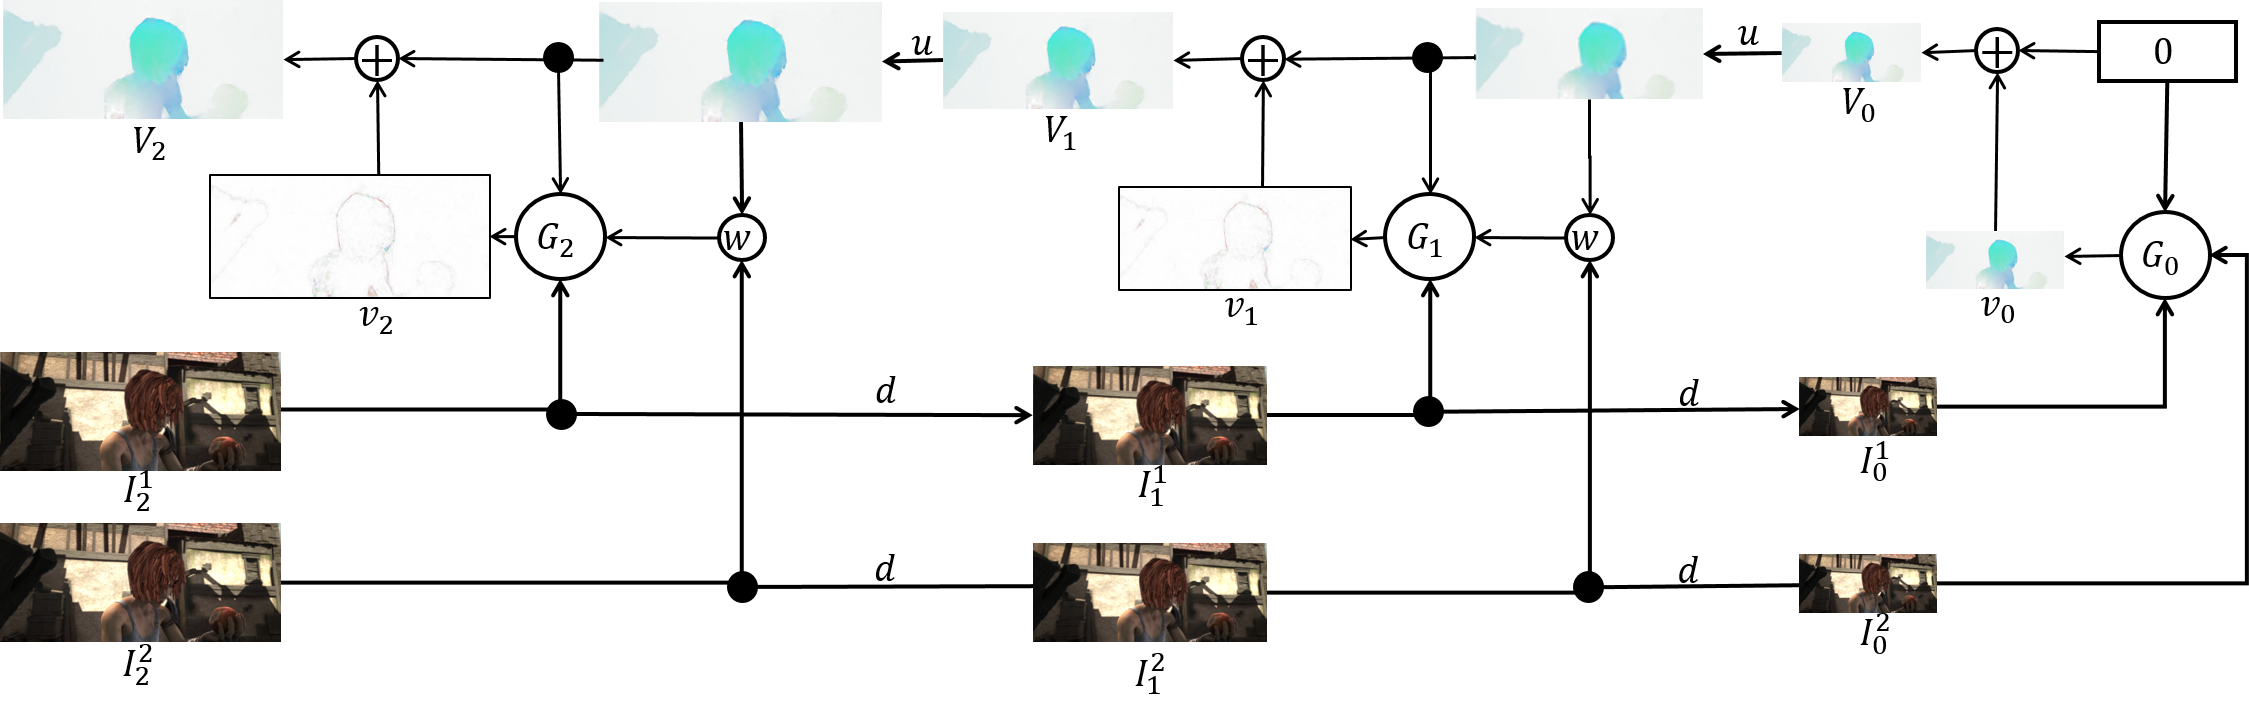
\includegraphics[width=\linewidth]{Infer2.png}
}
\caption{Inference in a 3-Level Pyramid Network \cite{denton2015deep}: The network $G_0$ computes the residual flow $v_0$ at the highest level of the pyramid (smallest image) using the low resolution images $\{I_0^1, I_0^2\}$. At each pyramid level, the network $G_k$ computes a residual flow $v_k$ which propagates to each of the next lower levels of the pyramid in turn, to finally obtain the flow $V_2$ at the highest resolution.}
\label{fig:infer}
\end{figure*}

\subsection{Spatial Sampling}
Let $d(\cdot)$ be the downsampling function that decimates an $m \times n$ image $I$ to the corresponding image $d(I)$ of size $m/2 \times n/2$. Let $u(\cdot)$ be the reverse operation that upsamples images. These operators are also used for downsampling and upsampling the horizontal and vertical components of the optical flow field, $V$. 
We also define a warping operator $w(I,V)$ that warps the image, $I$ according to the flow field, $V$, using  bi-linear interpolation.

\subsection{Inference}
Let $\{G_0, ... ,G_K\}$ denote a  set of trained convolutional neural network (convnet) models,
each of which computes residual flow, $v_k$
\begin{align}
v_k &= G_k(I_k^1, w(I_k^2,u(V_{k-1}) ), u(V_{k-1}))
\end{align}
at the $k$-th pyramid level. The convnet $G_k$ computes the residual flow $v_k$ using the upsampled flow from the previous pyramid level, ${V_{k-1}}$, and the frames $\{ I^1_k, I^2_k \}$ at level $k$. 
The second frame $I^2_k$ is warped using the flow as $w(I^2_k, u({V_{k-1}}))$ before feeding it to the convnet $G_k$. The flow, $V_k$ at the $k$-th pyramid level is then 
\begin{align}
\label{eq:flowprop}
V_k &= u(V_{k-1}) + v_k .
\end{align}
As shown in Fig.~\ref{fig:infer}, we start with downsampled images $\{ I_0^1, I_0^2\}$ and an initial flow estimate that is zero everywhere to compute the residual flow $v_0 = V_0$ at the top of the pyramid. We upsample the resulting flow, $u(V_0)$, and pass it to the network $G_1$ along with $\{I_1^1, w(I_1^2, u(V_0)) \}$ to compute the residual flow $v_1$. At each pyramid level, we compute the flow $V_k$ using Equation (\ref{eq:flowprop}). The flow $V_k$ is similarly propagated to higher resolution layers of the pyramid until we obtain the flow $V_K$ at full resolution. 
Figure \ref{fig:infer} shows the working of our approach using a 3-level pyramid. In experiments, we use a 5-level pyramid ($K=4$).

\begin{figure}[t]
\centerline{   
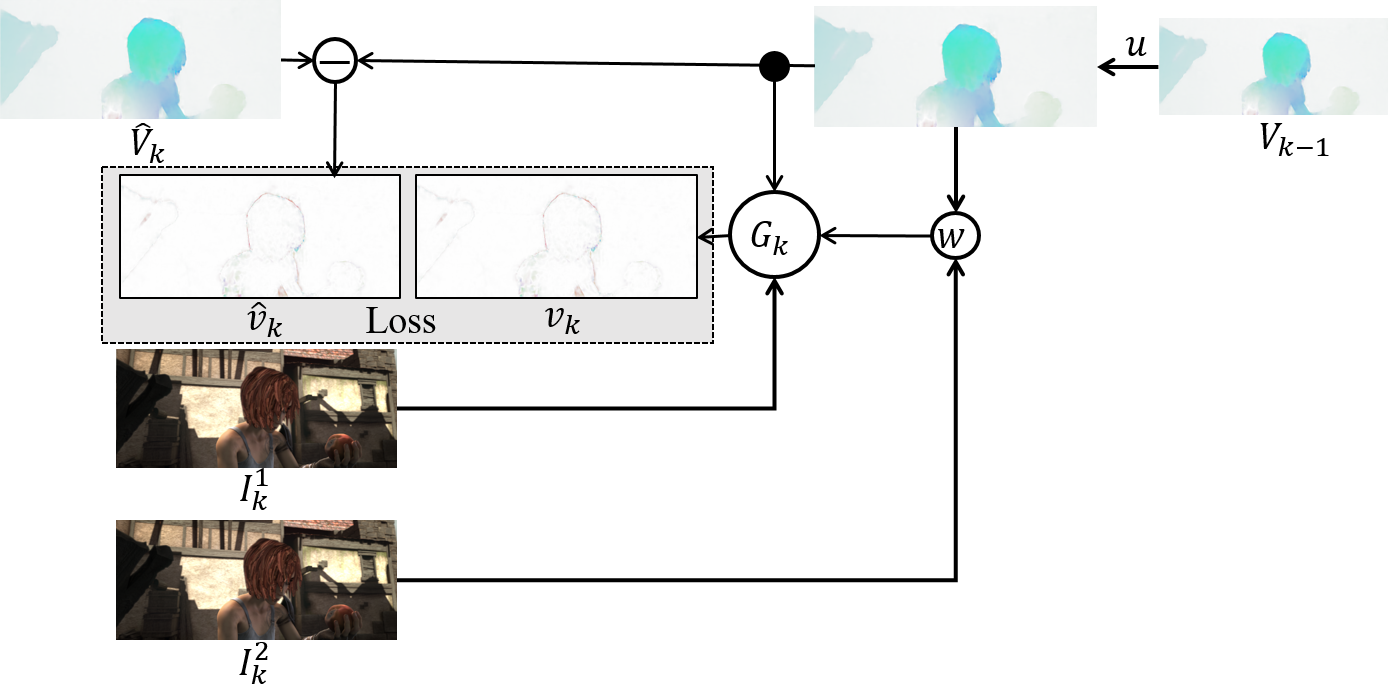
\includegraphics[width=\linewidth]{Train3.png}
}
%\vspace{-0.05in}
   \caption{Training network $G_k$ requires trained models $\{G_0 ... G_{k-1}\}$ to obtain the initial flow $u(V_{k-1})$. We obtain ground truth residual flows $\hat{v}_k$ by subtracting downsampled ground truth flow $\hat{V}_k$ and $u(V_{k-1})$ to train the network $G_k$ using the EPE loss.}
\label{fig:Train}
\end{figure}


\subsection{Training and Network Architecture}
We train each of the convnets $\{G_0,...,G_K\}$ independently and sequentially to compute the residual flow $v_k$ given the inputs $\{I_k^1, w(I_k^2,u(V_{k-1}) ), u(V_{k-1})\}$. We compute target residual flows $\hat{v}_k$ as a difference of target flow $V_k$ at the $k$-th pyramid level and the upsampled flow, $u(V_{k-1})$ obtained from the trained convnet of the previous level
\begin{align}
\hat{v}_k = \hat{V}_k - u(V_{k-1}) .
\end{align}
As shown in Fig.~\ref{fig:Train}, we train each of the networks, $G_k$, to minimize the average End Point Error (EPE) loss on the residual flow $v_k$.

%\subsection{Network Architecture and Details}
Each level in the pyramid has a simplified task relative to the full optical flow estimation problem; it only has to estimate a small-motion update to an existing flow field.
Consequently each network can be simple.
Here, each $G_k$ has 5 convolutional layers, which we found gave the best combination of accuracy, size, and speed.
We train five convnets $\{G_0, ..., G_4 \}$ at different resolutions of the Flying Chairs dataset. The network $G_0$ is trained with 24x32 images. We double the resolution at each lower level and finally train the convnet, $G_4$ with a resolution of 384x512.

Each convolutional layer is followed by a Rectified Linear Unit (ReLU), except the last one. 
We use a 7x7 convolutional kernel for each of the layers and found these work better than smaller filters.
The number of feature maps in each convnet, $G_k$ are \{32, 64, 32, 16, 2\}. The image $I^1_k$ and the warped image $w(I^2_k, u(V_{k-1}))$ have 3 channels each (RGB). The upsampled flow $u(V_{k-1})$ is 2 channel (horizontal and vertical).  
We stack image frames together with upsampled flow to form an 8 channel input to each $G_k$. The output is 2 channel flow corresponding to velocity in $x$ and $y$ directions. 

%We found that five layers gave the best combination of accuracy, size, and speed.
%We also found that 7x7 filters are better than smaller filters.
%Using fewer layers reduced accuracy, while using more did not produce improvements significant enough to justify the increased memory and run time.
%Fewer layers are insufficient due to lower receptive field, and large number of layers increases memory and speed constraints.

%\subsection{Implementation Details}
We train five networks $\{G_0, ..., G_4 \}$ such that each network $G_k$ uses the previous network $G_{k-1}$ as initialization. The networks are trained using Adam \cite{kingma2014adam} optimization with $\beta_1 = 0.9$ and $\beta_2 = 0.999$. We use a batch size of 32 across all networks with 4000 iterations per epoch. We use a learning rate of 1e-4 for the first 60 epochs and decrease it to 1e-5 until the networks converge. We use Torch7\footnote{\url{http://torch.ch/}} as our deep learning framework. We use the Flying Chairs \cite{dosovitskiy2015flownet} dataset and the MPI Sintel \cite{Butler:ECCV:2012} for training our network. 
All our networks are trained on a single Nvidia K80 GPU.

%\paragraph{Data Augmentation} 
We include various types of data augmentation during training. We randomly scale images by a factor of $[1, 2]$ and apply rotations at random within $[-17^{\circ}, 17^{\circ}]$. We then apply a random crop to match the resolution of the convnet, $G_k$ being trained. We include additive white Gaussian noise sampled uniformly from $\mathcal{N}(0, 0.1)$. We apply color jitter with additive brightness, contrast and saturation sampled from a Gaussian, $\mathcal{N}(0, 0.4)$. We finally normalize the images using a mean and standard deviation computed from a large corpus of ImageNet \cite{ILSVRC15} data in \cite{he2015deep}.

%-------------------------------------------------------------------------
\section{Experiments}
%-------------------------------------------------------------------------
\begin{figure}[t]
\begin{center}
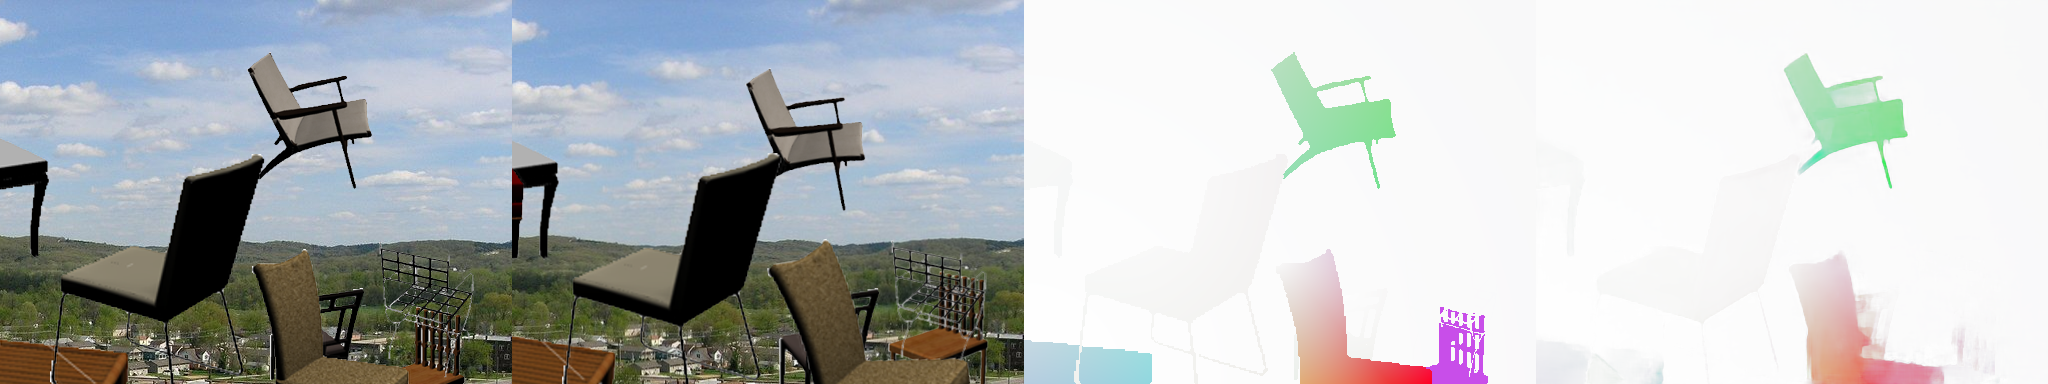
\includegraphics[width=\linewidth]{01119_viz.png}
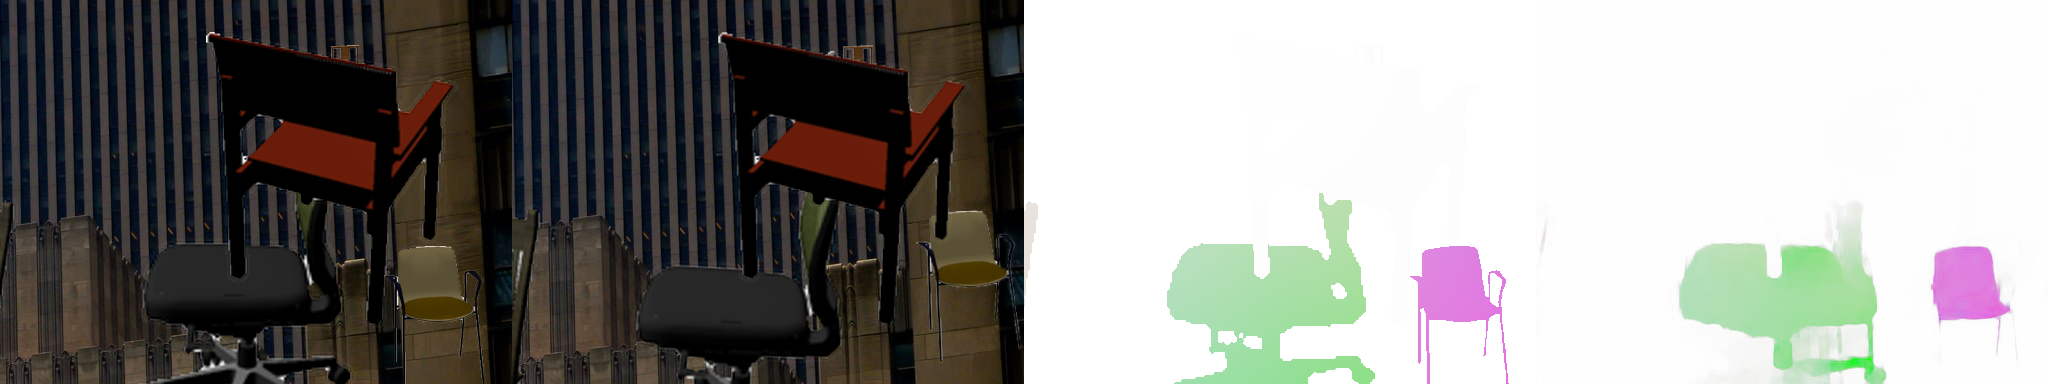
\includegraphics[width=\linewidth]{01519_viz.png}
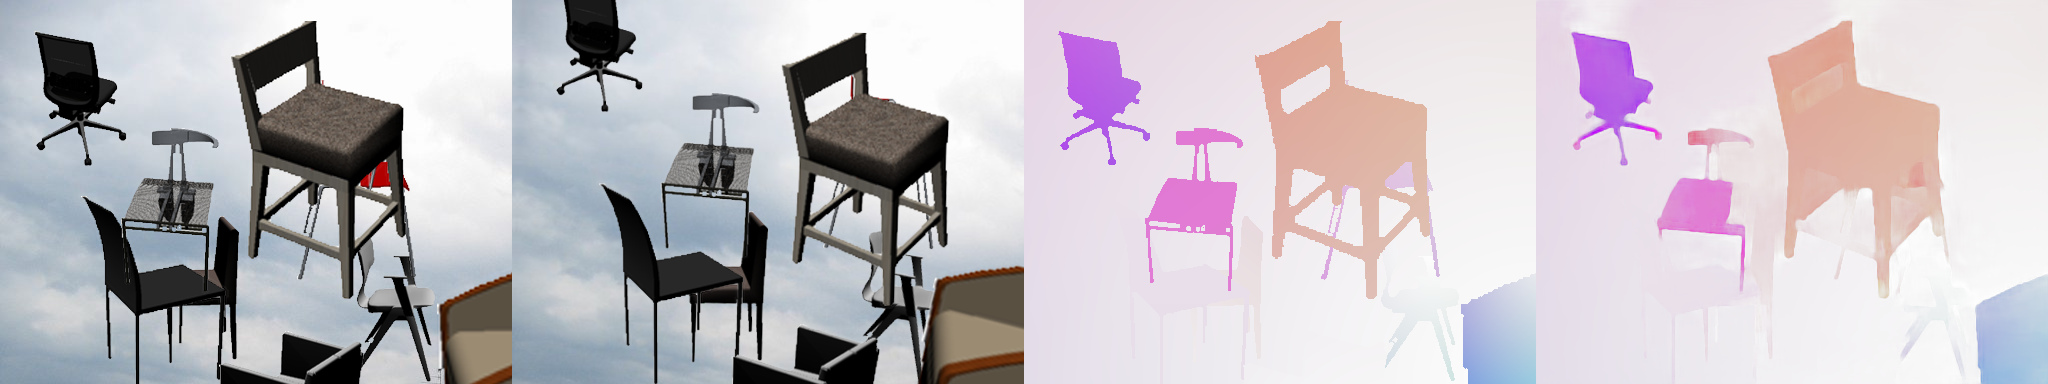
\includegraphics[width=\linewidth]{03273_viz.png}
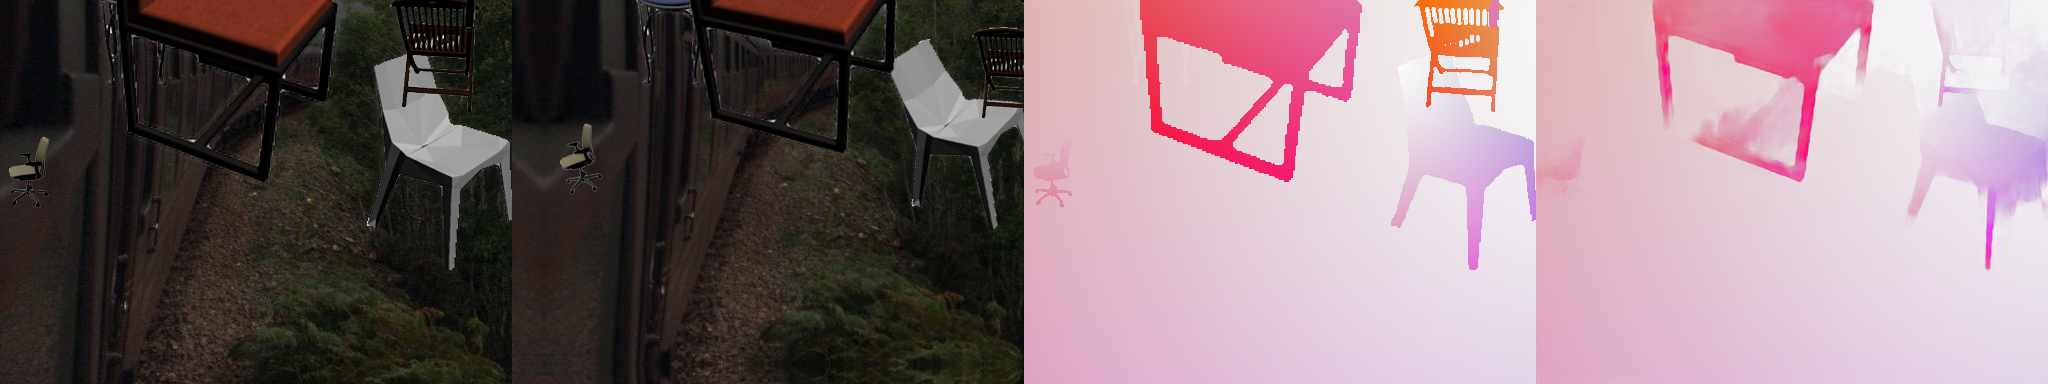
\includegraphics[width=\linewidth]{08658_viz.png}
\begin{tabular}{C{0.08\textwidth}C{0.09\textwidth}C{0.14\textwidth}C{0.07\textwidth}}
Frame 1 & Frame 2 & Ground Truth & SPyNet \\
 \end{tabular}
\end{center}
\vspace{-0.1in}
   \caption{Visualization of optical flow estimates using our model (SPyNet) and the corresponding ground truth flow fields on the Flying Chairs dataset.}
\label{fig:chairsresults}
\end{figure}


\begin{figure*}
\begin{center}
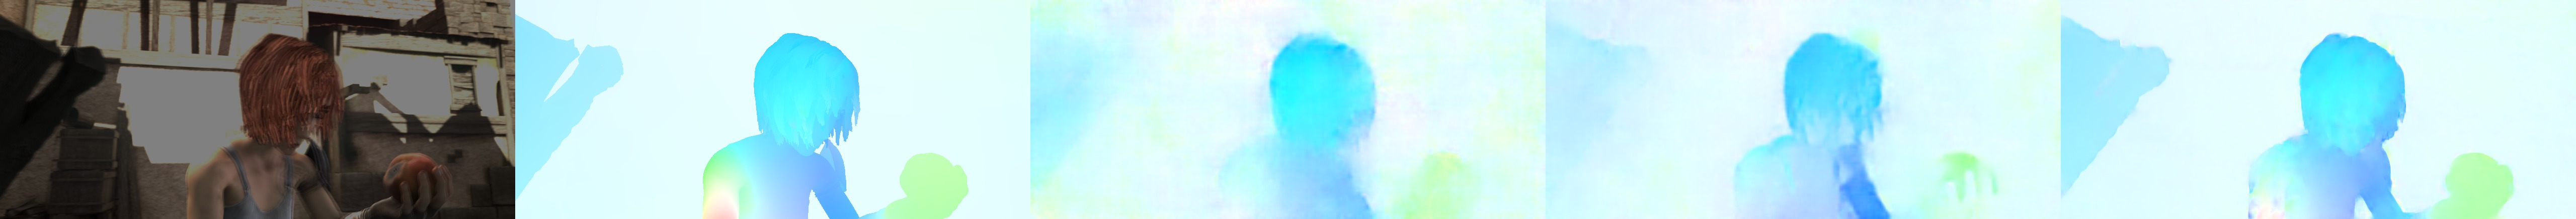
\includegraphics[width=\linewidth]{final3.jpg}
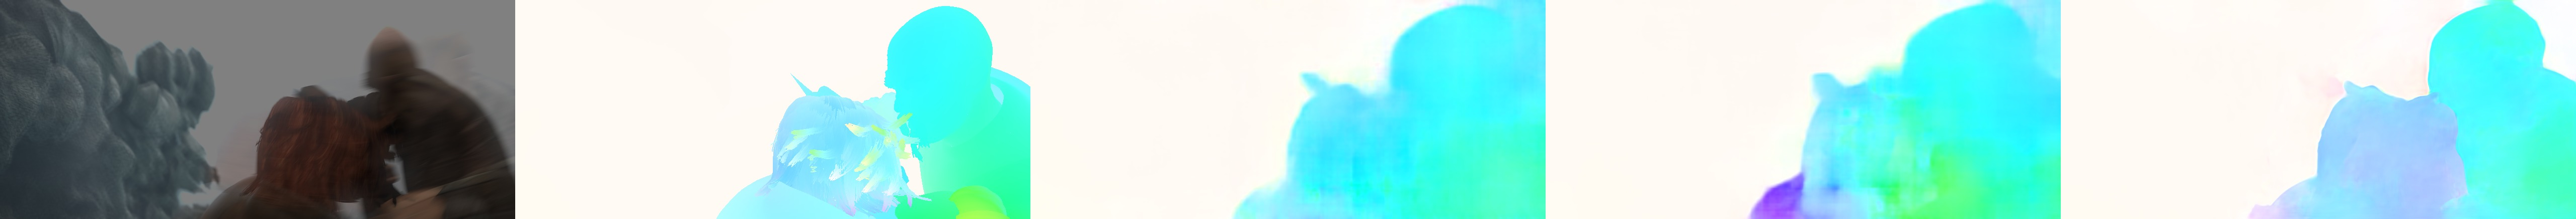
\includegraphics[width=\linewidth]{final196.jpg}
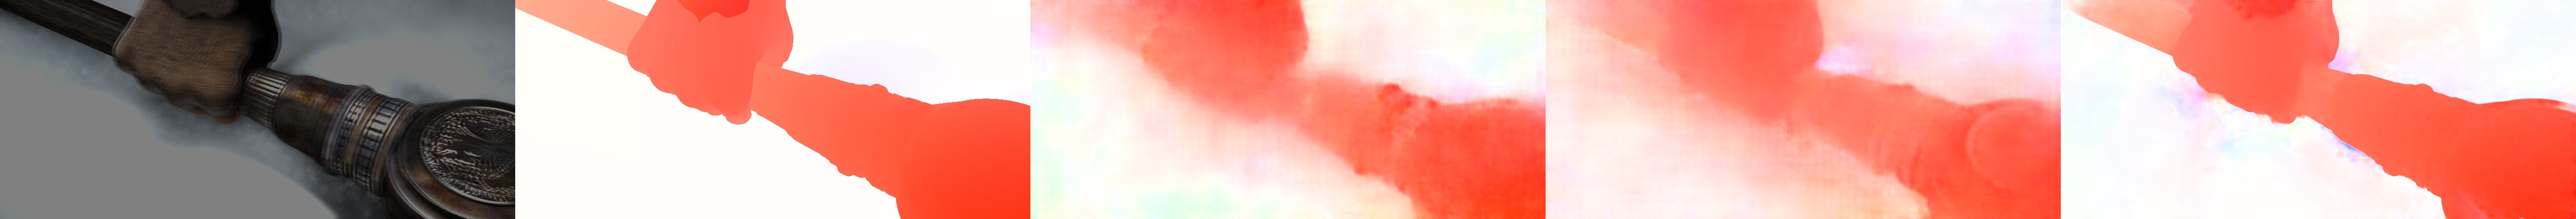
\includegraphics[width=\linewidth]{final253.jpg}
%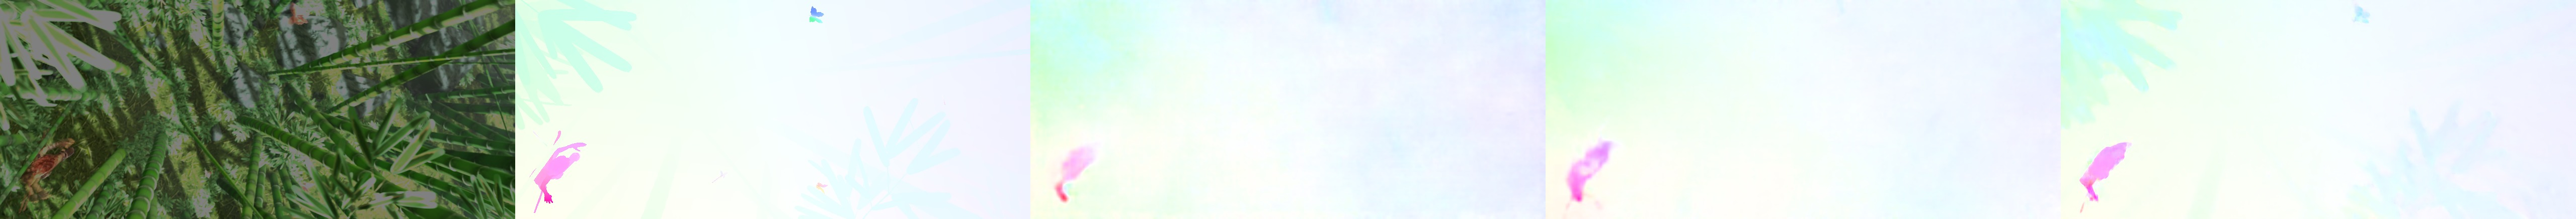
\includegraphics[width=\linewidth]{final268.png}
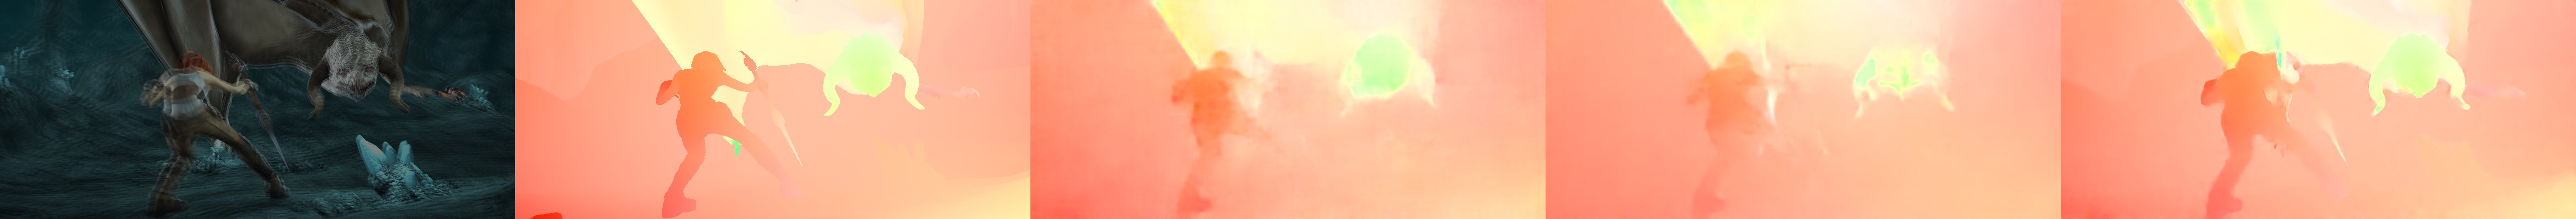
\includegraphics[width=\linewidth]{final512.jpg}
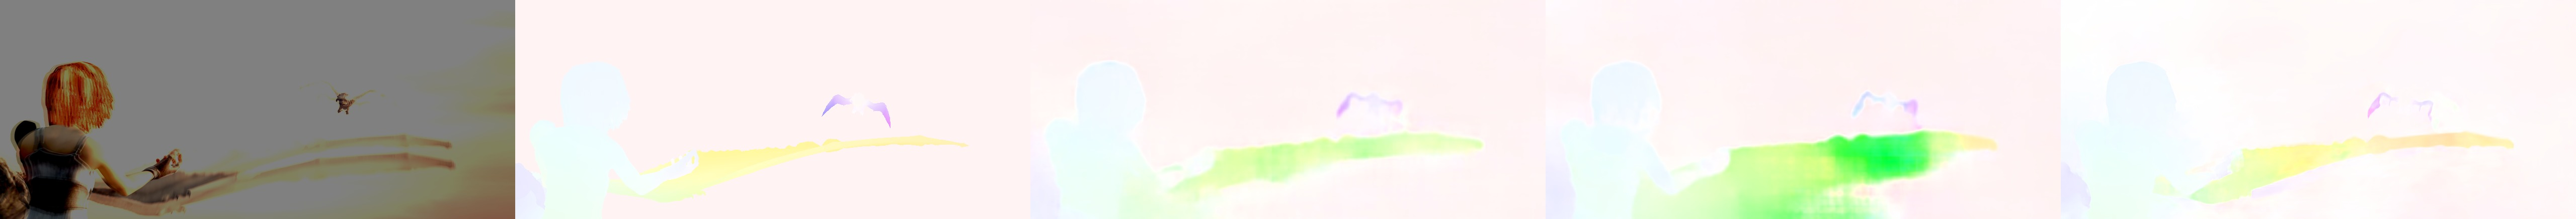
\includegraphics[width=\linewidth]{final993.jpg}
%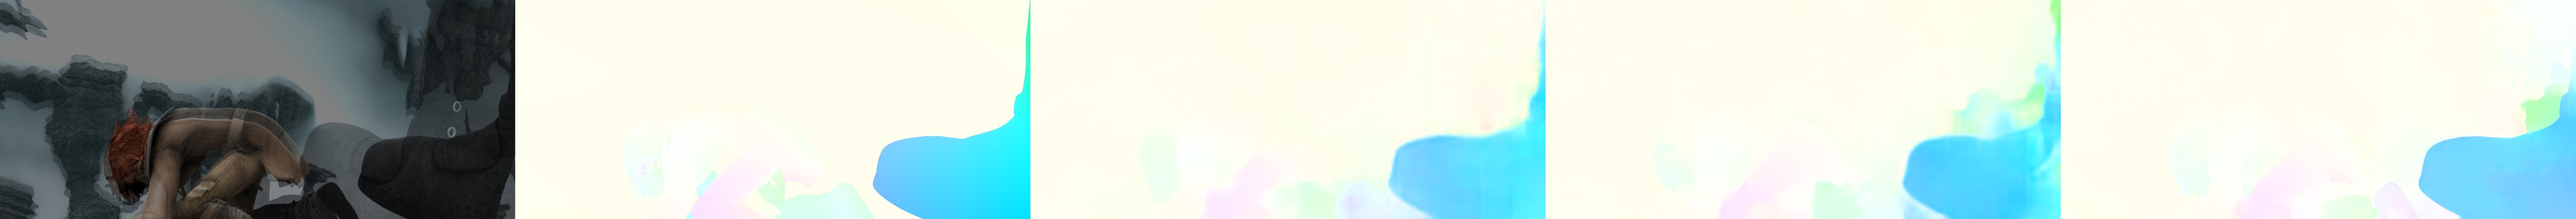
\includegraphics[width=\linewidth]{clean145.png}
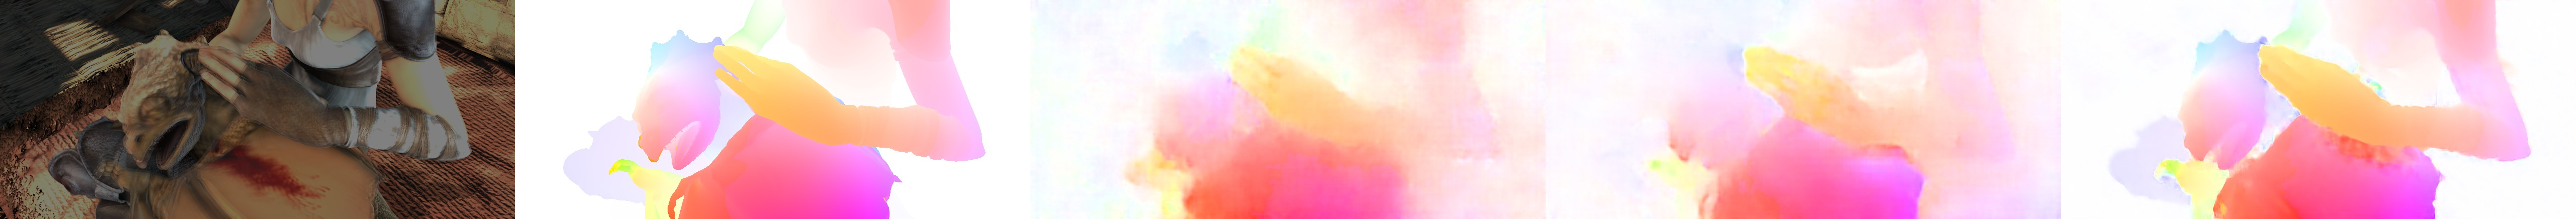
\includegraphics[width=\linewidth]{clean388.jpg}
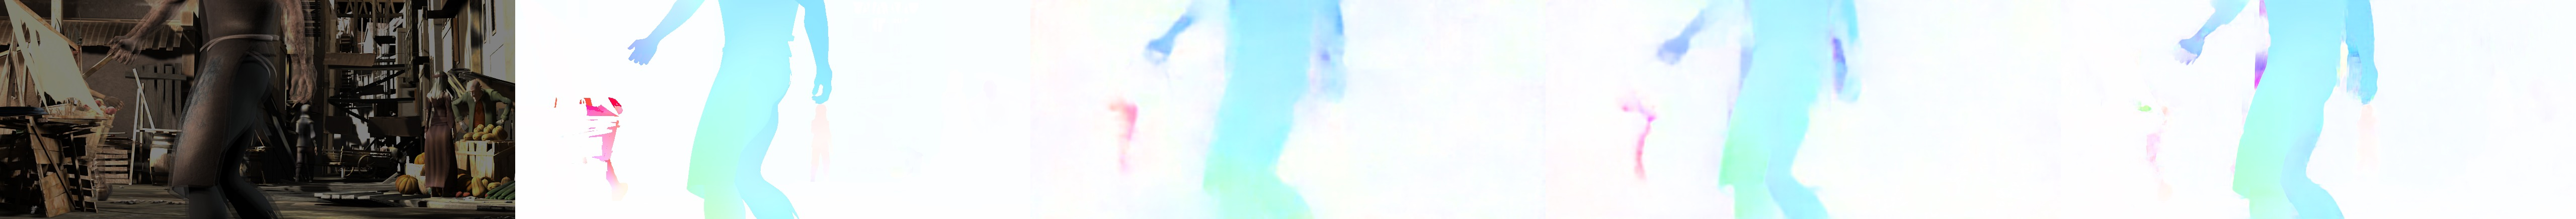
\includegraphics[width=\linewidth]{clean562.jpg}
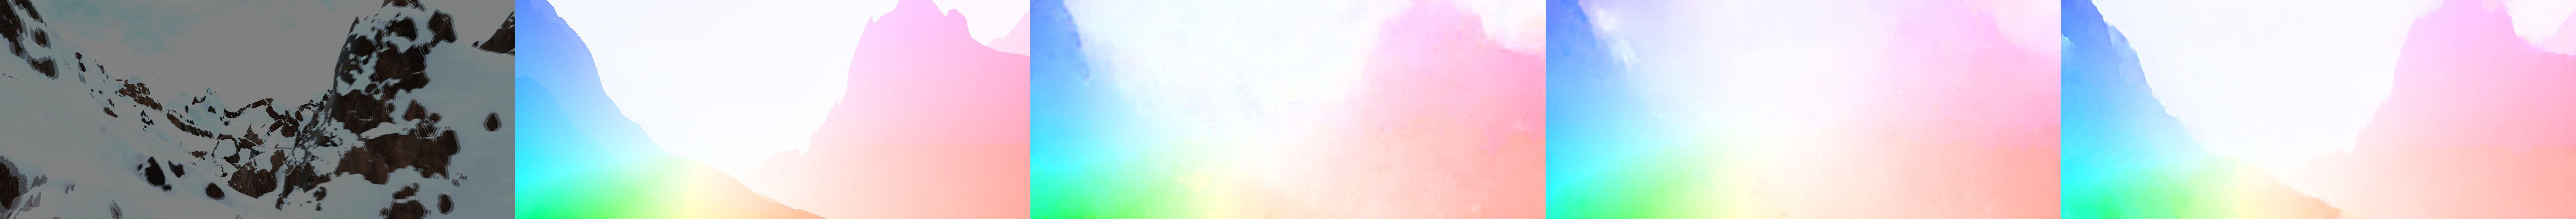
\includegraphics[width=\linewidth]{clean699.jpg}
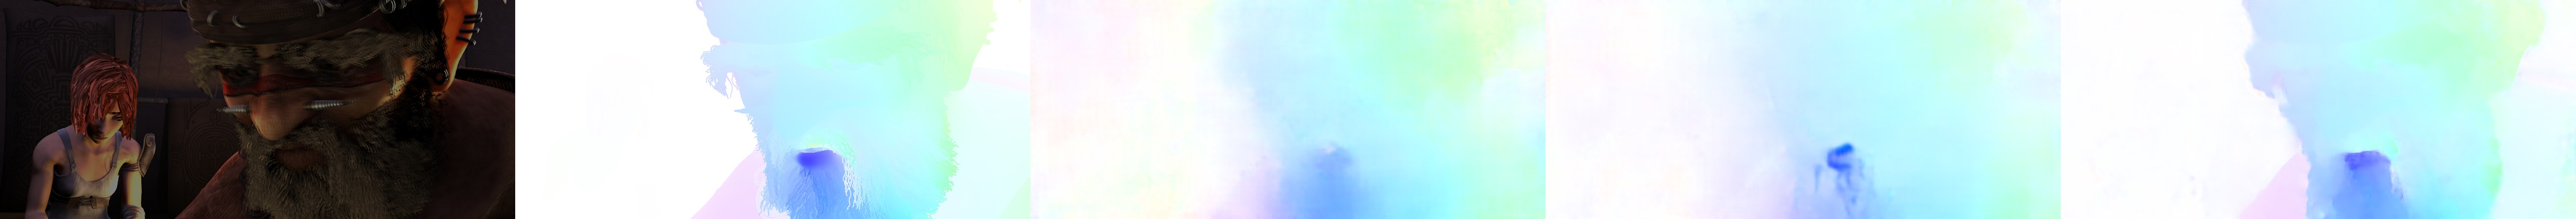
\includegraphics[width=\linewidth]{clean765.jpg}
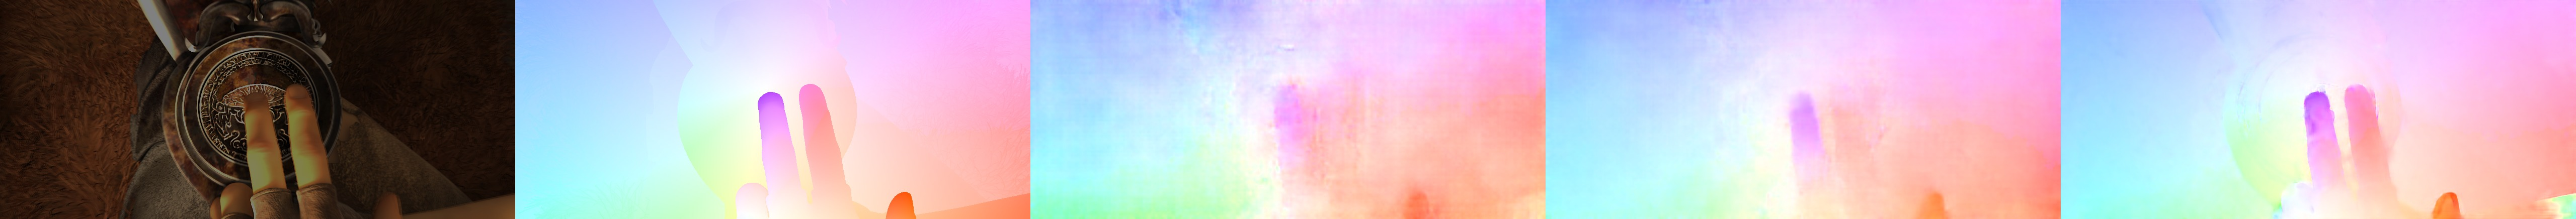
\includegraphics[width=\linewidth]{clean818.jpg}
\begin{tabular}{C{0.2\textwidth}C{0.16\textwidth}C{0.16\textwidth}C{0.16\textwidth}C{0.2\textwidth}}
Frames & Ground Truth & FlowNetS & FlowNetC & SPyNet \\
 \end{tabular}
\end{center}
\vspace{-0.1in}
\caption{Visual comparison of optical flow estimates using our  SPyNet model with FlowNet on the MPI Sintel dataset. The top five rows are from the  Sintel Final set and the bottom five row are from the Sintel Clean set.
SPyNet performs particularly well when the motions are relatively small.
}
\label{fig:sintelresults}
\end{figure*}

%-------------------------------------------------------------------------
\begin{table*}
\begin{center}
\begin{tabular}{lcccccccccc}
\Xhline{4\arrayrulewidth}
Method      & \multicolumn{2}{c}{\underline{Sintel Clean}} & \multicolumn{2}{c}{\underline{Sintel Final}} & \multicolumn{2}{c}{\underline{  \quad  KITTI \quad    }} & \multicolumn{2}{c}{\underline{Middlebury}} & \underline{Flying Chairs} & \multicolumn{1}{l}{Time (s)} \\
            & train            & test           & train            & test           & train        & test        & train           & test          & test          & \multicolumn{1}{l}{}   \\ \Xhline{4\arrayrulewidth}
Classic+NLP    & 4.13             & 6.73           & 5.90             & 8.29           & -         & -           & 0.22            & 0.32             & 3.93          & 102                         \\ \hline
FlowNetS    & 4.50             & 7.42           & \textbf{5.45}             & \textbf{8.43}           & \textbf{8.26}         & -           & 1.09            & -             & 2.71          & 0.080                         \\
FlowNetC    & 4.31             & 7.28           & 5.87             & 8.81           & 9.35         & -           & 1.15            & -             & \textbf{2.19}          & 0.150                         \\
SPyNet      & \textbf{4.12}             & \textbf{6.69}           & 5.57             & \textbf{8.43}           & 9.12         & -             & \textbf{0.33}            & \textbf{0.58}          & 2.63          & \textbf{0.069}                         \\ \hline
FlowNetS+ft & 3.66             & 6.96           & 4.44             & \textbf{7.76}           & 7.52         & 9.1         & 0.98            & -             & 3.04          & 0.080                         \\
FlowNetC+ft & 3.78             & 6.85           & 5.28             & 8.51           & 8.79         & -           & 0.93            &               & \textbf{2.27}          & 0.150                         \\
SPyNet+ft   & \textbf{3.17}             & \textbf{6.64}           & \textbf{4.32 }            & 8.36           & \textbf{4.13}         & \textbf{4.7}         & \textbf{0.33}            & \textbf{0.58}           & 3.07             & \textbf{0.069}                         \\  \Xhline{4\arrayrulewidth}
\end{tabular}
\end{center}
\caption{Average end point errors (EPE). Results are divided into methods trained with (+ft) and without fine tuning.  Bold font indicates the most accurate results among the convnet methods. All run times are measured on Flying Chairs and exclude image loading time.}
\label{tab:results}
\end{table*}

\begin{table*}
\begin{center}
\begin{tabular}{lcccccccccccc}
\Xhline{4\arrayrulewidth}
\multicolumn{1}{l}{Method} & \multicolumn{6}{c}{\underline{\qquad \qquad \qquad \quad Sintel Final \quad \qquad \qquad \qquad}} & \multicolumn{6}{c}{\underline{\qquad \qquad \qquad \quad Sintel Clean \quad \qquad \qquad \qquad}} \\ 
 & $d_{0\text{-}10}$ & $d_{10\text{-}60}$ & $d_{60\text{-}140}$ & $s_{0\text{-}10}$ & $s_{10\text{-}40}$ & $s_{40+}$ & $d_{0\text{-}10}$ & $d_{10\text{-}60}$ & $d_{60\text{-}140}$ & $s_{0\text{-}10}$ & $s_{10\text{-}40}$ & $s_{40+}$\\ \hline
FlowNetS+ft & 7.25 & 4.61 &\textbf{ 2.99} & 1.87 & 5.83 & 43.24 & 5.99 & 3.56 & 2.19 & 1.42 & 3.81 & 40.10 \\ 
FlowNetC+ft & 7.19 & 4.62 & 3.30 & 2.30 & 6.17 & \textbf{40.78} & 5.57 & 3.18 & 1.99 & 1.62 & 3.97 & \textbf{33.37 }\\ 
SpyNet+ft & \textbf{6.69} & \textbf{4.37} & 3.29 &\textbf{ 1.39} & \textbf{5.53 }& 49.71 & \textbf{5.50} & \textbf{3.12} & \textbf{1.71 }& \textbf{0.83} & \textbf{3.34 }& 43.44 \\ \Xhline{4\arrayrulewidth}
\end{tabular}
\end{center}
\caption{Comparison of FlowNet and SpyNet on the Sintel benchmark for different velocities, $s$, and distances, $d$, from motion boundaries.}
\label{tab:sintel}
\end{table*}

We evaluate our performance on standard optical flow benchmarks and compare with FlowNet \cite{dosovitskiy2015flownet}
and Classic+NLP \cite{sun2014quantitative}, a traditional pyramid-based method.
%We show better performance than FlowNet on most standard benchmarks with a 96\% reduction in model parameters.  
%We also compare with Classic+NLP, which is a traditional pyramid-based method and show significantly improved performance in most cases, while being three orders of magnitude faster.
We compare performance using average end point errors in Table \ref{tab:results}.
We evaluate on all the standard benchmarks and find that 
SPyNet is the most accurate overall, with and without fine tuning (details below).
%in 7 of the categories tested,  FlowNetS is most accurate in 3, and FlowNetC is most accurate in 1.
Additionally SPyNet is faster than all other methods. 
%SpyNet+ft fine-tuned on driving scenes \cite{sceneflowdataset} outperforms FlowNetS on KITTI by a big margin.

Note that the FlowNet results reported on the MPI-Sintel website are for a version that applies variational refinement (``+v'') to the convnet results.
Here we are not interested in the variational component and only compare the results of the convnet output.
%  which could be additionally applied to the output of any convnet with similar results.
% Consequently, here we compare only on results of the convnet output.

\paragraph{Flying Chairs.}
Once the convnets $G_k$ are trained on Flying Chairs, we fine tune the network on the same dataset but without any data augmentation at a learning rate of 1e-6. 
We see an improvement of EPE by 0.14 on the test set. 
Our model achieves better performance than FlowNetS \cite{dosovitskiy2015flownet} on the Flying Chairs dataset, however FlowNetC \cite{dosovitskiy2015flownet} performs better than ours. 
We show the qualitative results on Flying Chairs dataset in Fig.~\ref{fig:chairsresults} and compare the performance in Table \ref{tab:results}.

\paragraph{MPI-Sintel.}
The resolution of Sintel images is 436x1024. 
To use SPyNet, we scale the images to 448x1024, and use 6 pyramid levels to compute the optical flow. The networks used on each pyramid level are $\{G_0, G_1, G_2, G_3, G_4, G_4\}$. We repeat the network $G_4$ at the sixth level of pyramid for experiments on Sintel. 
Because Sintel has extremely large motions, we found that this gives better performance than using just five levels.

We evaluate the performance of our model on MPI-Sintel \cite{Butler:ECCV:2012} in two ways.
% Clean and Final, training and test sequences, with and without fine tuning.
First, we directly use the model trained on Flying Chairs dataset and evaluate our performance on both the training and the test sets. 
Second, we extract a validation set from the Sintel training set, using  the same partition as \cite{dosovitskiy2015flownet}. 
We fine tune our model independently on the Sintel Clean and Sintel Final split, and evaluate the EPE. 
The fine-tuned models are listed as ``+ft'' in Table \ref{tab:results}.
We show the qualitative results on MPI-Sintel in Fig.~\ref{fig:sintelresults}. 

Table \ref{tab:sintel} compares our fine-tuned model with FlowNet \cite{dosovitskiy2015flownet} for different velocities and distances from motion boundaries. 
We observe that SPyNet is more accurate than FlowNet for all velocity ranges  except the largest displacements (over 40 pixels/frame). 
%Our model suffers in large displacement regions over 40 pixels. 
SPyNet is also more accurate than FlowNet close to motion boundaries, which is important for many problems.  %at all distances from motion boundaries except when greater than 60 pixels away.
%We also underperform in occluding regions which are greater than 60 pixels away from the object boundary. 

\paragraph{KITTI and Middlebury.}
We evaluate KITTI \cite{Geiger2012CVPR} scenes using the base model SPyNet trained on Flying Chairs. 
We then fine-tune the model on Driving and Monkaa scenes from \cite{sceneflowdataset} and evaluate the fine-tuned model SPyNet+ft. 
Fine tuning results in a significant improvement in accuracy by about 5 pixels.
The large improvement in accuracy suggests that better training datasets are needed and that these could improve the accuracy of SPyNet further on general scenes.
 While SPyNet+ft is much more accurate than FlowNet+ft, the latter is fine-tuned on different data.

For the Middlebury \cite{baker2011database} dataset, we evaluate the sequences using the base model SPyNet
as well as SPyNet+ft,  which is fine-tuned on the  Sintel-Final dataset;  the Middlebury dataset itself is too small for fine-tuning. 
SPyNet is significantly more accurate on Middlebury, where FlowNet has trouble with the small motions.
Both learned methods are less accurate than Classic+NL on Middlebury but both are also significantly faster.



\section{Analysis}
%We evaluate the performance of our model in terms of its size, speed,
%and accuracy.
% in comparison to previous optical flow methods. We compare our model size with previous deep networks and interpret the our learned filters.


\paragraph{Model Size}
Combining spatial pyramids with convnets results in a huge reduction in model complexity.
% We analyze the size of our model that can capture the distribution of functions for estimating optical flow. The model size is the total number of parameters that are learned by the model. We compare our model with the previous state of the art methods in end-to-end deep learning for optical flow estimation. 
At each pyramid level, a network, $G_k$, has 240,050 learned parameters.
The total number of parameters learned by the entire network is 1,200,250, with 5 spatial pyramid levels.
In comparison, FlowNetS and FlowNetC \cite{dosovitskiy2015flownet} have 32,070,472 and 32,561,032 parameters respectively. 
SPyNet is about 96 \% smaller than FlowNet (Fig.~\ref{fig:modelSize}).
\begin{figure}[t]
\centerline{
   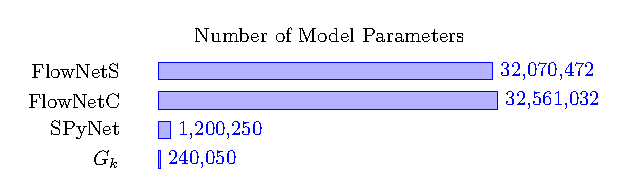
\includegraphics[width=\linewidth]{modelSize.pdf}
}
   \caption{Model size of various methods. Our model is 96\% smaller
     than the previous state-of-the-art flow method trained using end-to-end deep learning.}
\label{fig:modelSize}
\end{figure}

The spatial pyramid approach enables a significant reduction in model parameters without sacrificing accuracy. 
There are two reasons -- the warping function and learning of residual flow. 
%The warping function is a non-linear function that stretches and squeezes the image according to the flow field. 
%It has been used widely in the optical flow literature \cite{sun2014quantitative} to achieve state of the art performance. 
%It might be possible to learn this function with several layers of a convolution network and enough data.
By using the warping function directly, the convnet does not need to
learn it. %reduce the parameters require to model it in a convnet. 
More importantly, the residual learning restricts the range of flow fields in the output space. 
Each network only has to model a smaller range of velocities at each level of the spatial pyramid. 
%Thus, we reduce the model size required for the entire range of flow fields.

SPyNet also has a small memory footprint. 
The disk space required to store all the model parameters is 9.7
MB. 
This could simplify deployment on mobile or embedded devices with GPU support.
%As a feedforward deep network, our models could run in real-time on phones and small devices.  

\begin{figure}[t]
\begin{center}
\subfigure[]{\label{fig:level1layer1}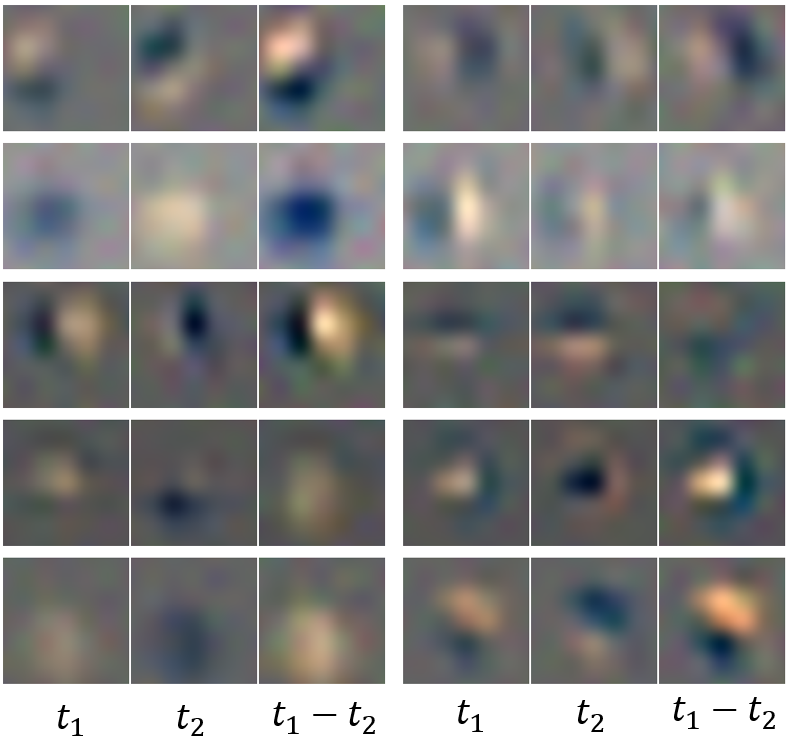
\includegraphics[width=0.485\linewidth]{level1layer1.png}}
~
\subfigure[]{\label{fig:fiterEvolution}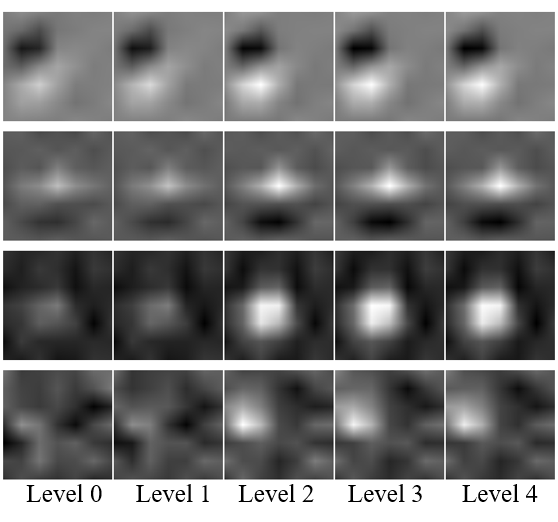
\includegraphics[width=0.485\linewidth]{filterEvolution.png}}
\end{center}     %%% not \center
\vspace{-0.1in}
\caption{(a) Visualization of filter weights in the first layer of $G_2$ showing their spatiotemporal nature on RGB image pairs. (b) Evolution of filters across the pyramid levels (from low resolution (0) to high resolution (4))}
\end{figure}
%\begin{figure}[t!]
%\begin{center}
%\begin{subfigure}[t]{0.5\linewidth}
%\centering
%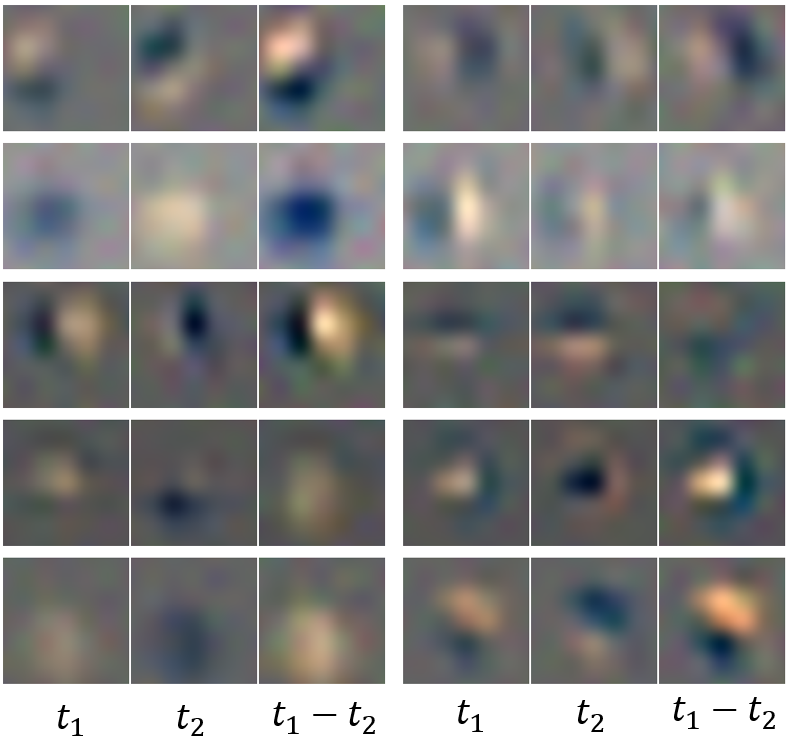
\includegraphics[]{level1layer1.png}
%	\begin{tabular}{C{0.055\textwidth}C{0.05\textwidth}C{0.065\textwidth}C{0.07\textwidth}C{0.03\textwidth}C{0.05\textwidth}}
%$t_1$ & $t_2$ & $t_1 - t_2$ & $t_1$ & $t_2$ & $t_1 - t_2$ \\
%	\end{tabular}
%\end{subfigure}
%~
%\begin{subfigure}[t]{0.5\linewidth}
%\centering
%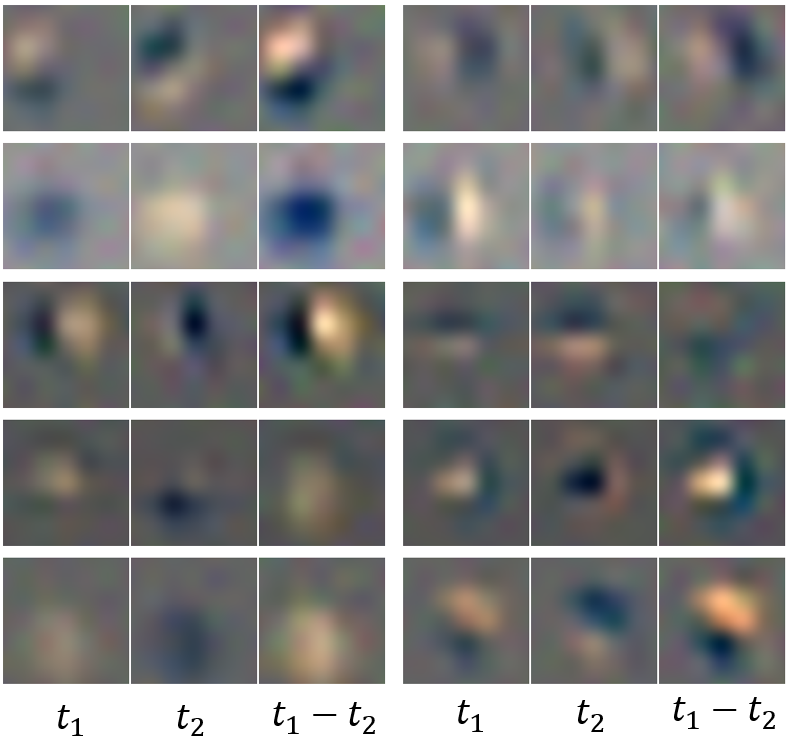
\includegraphics[]{level1layer1.png}
%	\begin{tabular}{C{0.055\textwidth}C{0.05\textwidth}C{0.065\textwidth}C{0.07\textwidth}C{0.03\textwidth}C{0.05\textwidth}}
%$t_1$ & $t_2$ & $t_1 - t_2$ & $t_1$ & $t_2$ & $t_1 - t_2$ \\
%	\end{tabular}
%\end{subfigure}
%\end{center}
%   \caption{Visualization of filter weights in the first layer of $G_2$ showing their spatiotemporal nature on RGB image pair.}
%\label{fig:level1layer1}
%\end{figure}
%We observe the filters learned by the neural network by visualizing their spatio-temporal components. 
%%%To gain insight into the method and to relate it to prior work on optical flow, we explore the filters learned by the network.
\paragraph{Visualization of Learned Filters.}
 Figure \ref{fig:level1layer1} shows examples of  filters learned by the first layer of the network, $G_2$. 
In each row, the first two columns show the spatial filters that operate on the RGB channels of the two input images respectively. 
The third column is the difference between the two spatial filters hence representing the temporal features learned by our model. 
We observe that most of the spatio-temporal filters in Fig.~\ref{fig:level1layer1} are equally sensitive to all color channels, and hence appear mostly grayscale.
Note that the actual filters are $7\times\/ 7$ pixels and are upsampled for visualization.
 
We observe that many of the spatial filters appear to be similar to traditional Gaussian derivative filters used by classical methods.
These classical filters are hand crafted and typically are applied in the horizontal and vertical direction.
Here, we observe a greater variety of derivative-like filters of varied scales and orientations.
We also observe filters that spatially resemble second derivative or Gabor filters \cite{adelson1985spatiotemporal}.
The temporal filters show a clear derivative-like structure in time.
Note that these filters are very different from those reported in \cite{dosovitskiy2015flownet} (Sup. Mat.), which have a high-frequency structure, unlike classical filters. 

Figure \ref{fig:fiterEvolution} illustrates how filters learned by the network at each level of the pyramid differ from each other. 
Recall that, during training, each network is initialized with the network before it in the pyramid.
The filters, however, do not stay exactly the same with training.
Most of the filters in our network look like rows 1 and 2, where the filters become sharper as we progress towards the finer-resolution levels of the pyramid. 
%As we proceed to finer levels of the pyramid, the filters become sharper to capture the spatial derivatives at higher resolution.  
However, there are some filters that are similar to rows 3 and 4, where these filters become more defined at higher resolution levels of the pyramid. 
%We believe that this might be a result of the filter becoming sensitive to image features that are significant only at high resolutions. 
%There are very few filters that appear to change completely across the pyramid levels as seen in rows 5 and 6. 
%These are the filters which respond to different features across the
%different resolution scales. 

%\begin{figure}[t]
%\begin{center}
%   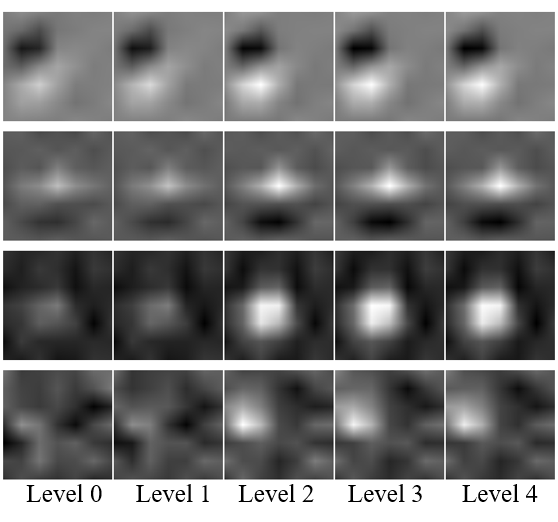
\includegraphics[width=\linewidth]{filterEvolution.png}
%   \begin{tabular}{C{0.07\textwidth}C{0.07\textwidth}C{0.07\textwidth}C{0.07\textwidth}C{0.08\textwidth}}
%Level 0 & Level 1 & Level 2 & Level 3 & Level 4 \\
% \end{tabular}
%\end{center}
%   \caption{Evolution of filters across the pyramid levels (from low resolution (0) to high resolution (4))}
%\label{fig:fiterEvolution}
%\end{figure}


\begin{figure}[t]
\centerline{
%   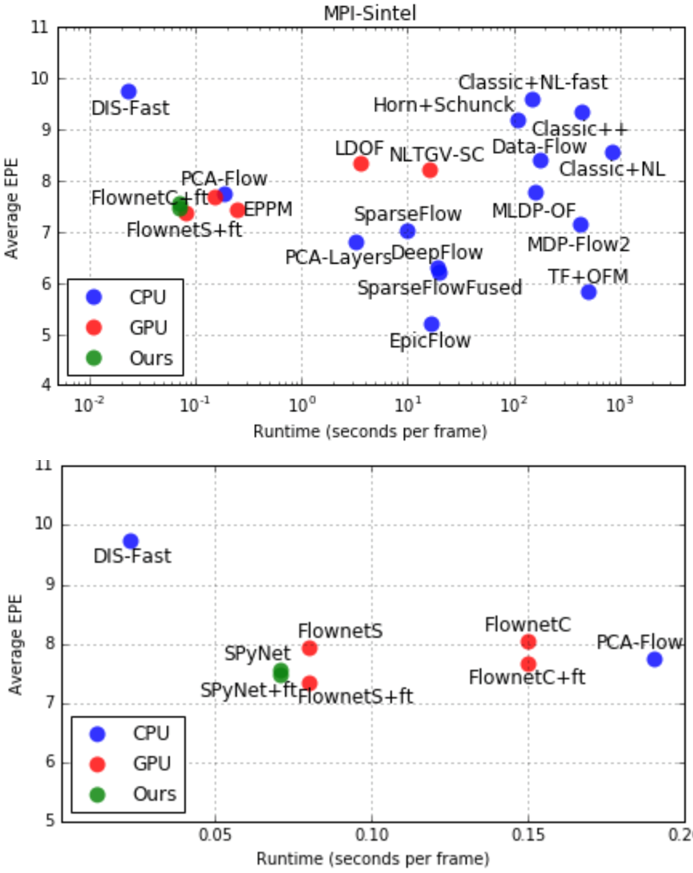
\includegraphics[width=\linewidth]{epevtime.png}
   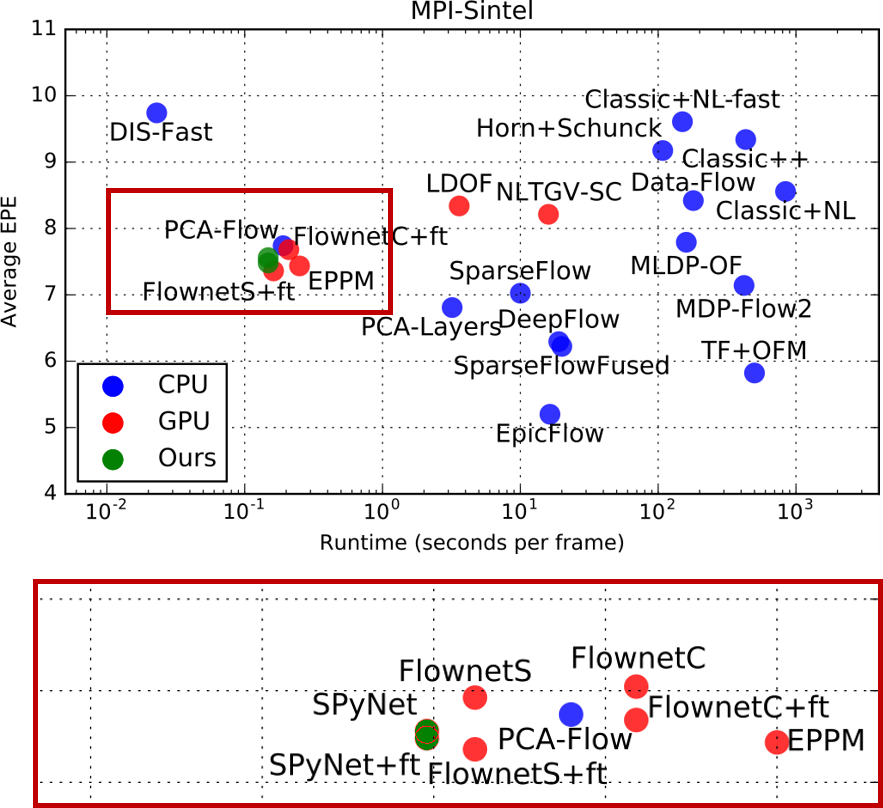
\includegraphics[width=0.8\linewidth]{epevtime2.png}
}
   \caption{Average EPE vs. runtime on MPI-Sintel. 
Zoomed in version on the bottom shows the fastest methods. Times were measured by us. Adapted from \cite{wulff2015efficient}. }
\label{fig:epevtime}
\end{figure}

\paragraph{Speed.}
 Optical flow estimation is traditionally viewed as an optimization problem involving some form of variational inference.
%either continuous or discrete \cite{sun2014quantitative}. 
Such algorithms are  computationally expensive, often taking several seconds or minutes per frame.
This has limited the application of optical flow in robotics, embedded systems, and video analysis.

Using a GPU can speed up traditional methods \cite{sundaram2010dense,Werlberger2009:GPUflow} but with reduced accuracy.
Feed forward deep networks \cite{dosovitskiy2015flownet} leverage fast
GPU convolutions and avoid iterative optimization.
%to speed up computations and look like the most promising methods to balance speed and accuracy.
Of course for embedded applications, network size is critical (see Fig.~\ref{fig:modelSize}).
%However, as the size of the network increases, the runtime becomes longer. We have also seen the use of basis vectors for flow \cite{wulff2015efficient} for improving speeds. 
% such as PCA-Flow \cite{wulff2015efficient} and FlowNet \cite{dosovitskiy2015flownet}. 
Figure \ref{fig:epevtime} shows the speed-accuracy comparisons of several well known methods.
All times shown are measured with the images already loaded in the memory. 
The errors are computed as the average EPE of both the clean and final MPI-Sintel sequences. 
%Our model can compute optical flow at 7ms/frame giving it ten times
%speed up over FlowNet. As such, it can be use for real time
%applications.
SPyNet offers a good balance between speed and accuracy; no
faster method  is as accurate.
 % is the fastest optical flow method with an accuracy in the range of popular methods.

\section{Discussion and Future Work}
Traditional flow methods linearize the brightness constancy equation resulting in an optical flow constraint equation
implemented with spatial and temporal derivative filters.
Sometimes methods adopt a more generic filter constancy assumption \cite{adelson1984pyramid,brox2004high}.
%These methods all rely on iterative minimization of an error function.
Our filters are somewhat different.  
% Instead of a small number, we learn a large filter bank and use them differently.
% There is no explicit iterative optimization.  
The filters learned by SPyNet are used in the direct computation of the flow by the feed-forward network.  
% Imagine a set of varied, shifted, and rotated filters.  
% The responses of the set will vary with the underlying motion.  
% This larger set of responses contrains the possible flow that could have produced them.  

%We also note that there is a long literature on learning or modeling filters for optical flow \cite{scharr2007optimal}.
%We note that our first level 7x7 filters typically have a larger spatial extent than most filters currently used on optical flow methods.

SPyNet is small compared with other recent optical flow networks.
Examination of the filters, however, suggests that it might be possible to make it significantly smaller still.
Many of the filters resemble derivative of Gaussian filters or Gabor filters at various scales, orientations, spatial frequencies, and spatial shifts.
Given this, it may be possible to significantly compress the filter bank by using dimensionality reduction or by using a set of analytic spatio-temporal features.
Some of the filters may also be separable.

Early methods for optical flow used analytic spatio-temporal features but, at the time, did not produce good results and the general line of spatio-temporal filtering decayed.
The difference from early work is that our approach suggests the need for a large filter bank of varied filters.
Note also that these approaches considered only the first convolutional layer of filters and did not seek a ``deep'' solution. 
This all suggests the possibility that a deep network of analytic filters could perform well.  
This could vastly reduce the size of the network and the number of parameters that need to be learned.
%In the spatial domain, for example, there is work relating the filters of convnets to wavelets \cite{Mallat20150203}.

Note that pyramids have well-known limitations for dealing with large motions \cite{brox2009large,Sevilla:ECCV:2014}.
In particular, small or thin objects that move quickly effectively disappear at coarse pyramid levels, making it impossible to capture their motion.
Recent approaches for dealing with such large motions use sparse matching to augment standard pyramids \cite{brox2009large,weinzaepfel2013deepflow}.
Future work should explore adding long-range matches to SPyNet.
%This suggests training a separate network for the task of large motion estimation and combining this with our SPyNet.
Alternatively Sevilla et al.~\cite{Sevilla:ECCV:2014} define a channel constancy representation that preserves fine structures in a pyramid.
The channels effectively correspond to filters that could be learned.

%\paragraph{Future Work.}
A spatial pyramid can be thought of as the simple application of a set of linear filters.
Here we take a standard spatial pyramid but one could learn the filters for the pyramid itself.
SPyNet also uses a standard warping function to align images using the flow computed from the previous pyramid level. 
This too could be learned. 

%Here we trained the network in a sequential fashion.  
%Better results are likely if the full network can be trained end-to-end.
%The pyramid down- and up-sampling operations linear functions so they are easy to learn.
%Image warping, however, is non-linear in the optical flow, complicating the propagation of
%derivatives through the full pyramid and all the networks.

% We could also make use of a layered flow approach \cite{Sun:CVPR:2013} to simultaneously learn flow and segmentation. 
% These are interesting directions for future research.
%Explicitly predict the occlusions and use these.

An appealing feature of SPyNet is that it is small enough to fit on a mobile device.  
Future work will explore a mobile implementation and its applications.
Additionally, we will explore extending the method to use more frames (e.g.~3 or 4).  
%This should enable the model to learn richer temporal filters and, for small motions, this might lead to more accurate results.
Multiple frames could enable the network to reason more effectively about occlusion.

Finally, Flying Chairs is not representative of natural scene motions, containing many huge displacements.
%may not be the best dataset for learning our network since it contains many huge displacements that are too large for classical pyramid approaches to capture.
%Such motions occur in animated films like Sintel but less often in real scenes.
We are exploring new training datasets to improve performance on common sequences where the motion is less dramatic.
%\myworries{Anurag's notes:}
%Optical Flow is interesting problem for deep learning. One of the few problems where output space is both continuous and dense.
\section{Conclusions}
In summary, we have described a new optical flow method that combines features of classical optical flow algorithms with deep learning.
In a sense, there are two notions of ``deepness'' here.
First we use a ``deep'' spatial pyramid to deal with large motions.
Second we use deep neural networks at each level of the spatial pyramid and train them to estimate a flow {\em update} at each level.
This approach means that each network has less work to do than a fully generic flow method that has to estimate arbitrarily large motions.
At each pyramid level we assume that the motion is small (on the order of a pixel).
This is borne out by the fact that the network learns spatial and temporal filters that resemble classical derivatives of Gaussians and Gabors.
Because each sub-task is so much simpler, our network needs many fewer parameters than previous methods like FlowNet.
This results in a method with a small memory footprint %that is small enough to fit on the phone and
that is faster than existing methods.
At the same time, SPyNet achieves an accuracy comparable to FlowNet, surpassing it in several benchmarks. 
This opens up the promise of optical flow that is both accurate, practical, and widely deployable.


\section*{Acknowledgement}
We thank Jonas Wulff for his insightful discussions about optical flow. 

%{\small
%\bibliographystyle{ieee}
%}
\begin{thebibliography}{10}\itemsep=-1pt

\bibitem{adelson1984pyramid}
E.~H. Adelson, C.~H. Anderson, J.~R. Bergen, P.~J. Burt, and J.~M. Ogden.
\newblock Pyramid methods in image processing.
\newblock {\em RCA engineer}, 29(6):33--41, 1984.

\bibitem{adelson1985spatiotemporal}
E.~H. Adelson and J.~R. Bergen.
\newblock Spatiotemporal energy models for the perception of motion.
\newblock {\em J.~Opt.~Soc.~Am.~A}, 2(2):284--299, Feb. 1985.

\bibitem{ahmadi2016unsupervised}
A.~Ahmadi and I.~Patras.
\newblock Unsupervised convolutional neural networks for motion estimation.
\newblock {\em arXiv preprint arXiv:1601.06087}, 2016.

\bibitem{baker2011database}
S.~Baker, D.~Scharstein, J.~Lewis, S.~Roth, M.~J. Black, and R.~Szeliski.
\newblock A database and evaluation methodology for optical flow.
\newblock {\em International Journal of Computer Vision}, 92(1):1--31, 2011.

\bibitem{bao2014tipeppm}
L.~Bao, Q.~Yang, and H.~Jin.
\newblock Fast edge-preserving {PatchMatch} for large displacement optical
  flow.
\newblock {\em Image Processing, IEEE Transactions on}, 23(12):4996--5006, Dec
  2014.

\bibitem{barron94-ijcv}
J.~Barron, D.~J. Fleet, and S.~S. Beauchemin.
\newblock Performance of optical flow techniques.
\newblock {\em Int. J. Comp. Vis. (IJCV)}, 12(1):43--77, 1994.

\bibitem{black1993framework}
M.~J. Black and P.~Anandan.
\newblock A framework for the robust estimation of optical flow.
\newblock In {\em Computer Vision, 1993. Proceedings., Fourth International
  Conference on}, pages 231--236. IEEE, 1993.

\bibitem{brox2009large}
T.~Brox, C.~Bregler, and J.~Malik.
\newblock Large displacement optical flow.
\newblock In {\em Computer Vision and Pattern Recognition, 2009. CVPR 2009.
  IEEE Conference on}, pages 41--48. IEEE, 2009.

\bibitem{brox2004high}
T.~Brox, A.~Bruhn, N.~Papenberg, and J.~Weickert.
\newblock High accuracy optical flow estimation based on a theory for warping.
\newblock In {\em European conference on computer vision}, pages 25--36.
  Springer, 2004.

\bibitem{burt-adelson}
P.~J. Burt and E.~H. Adelson.
\newblock The {Laplacian} pyramid as a compact image code.
\newblock {\em IEEE Transactions on Communications}, COM-34(4):532--540, 1983.

\bibitem{Butler:ECCV:2012}
D.~J. Butler, J.~Wulff, G.~B. Stanley, and M.~J. Black.
\newblock A naturalistic open source movie for optical flow evaluation.
\newblock In {A. Fitzgibbon et al. (Eds.)}, editor, {\em European Conf. on
  Computer Vision (ECCV)}, Part IV, LNCS 7577, pages 611--625. Springer-Verlag,
  Oct. 2012.

\bibitem{cadieu2008learning}
C.~Cadieu and B.~A. Olshausen.
\newblock Learning transformational invariants from natural movies.
\newblock In {\em Advances in neural information processing systems}, pages
  209--216, 2008.

\bibitem{chen2014semantic}
L.-C. Chen, G.~Papandreou, I.~Kokkinos, K.~Murphy, and A.~L. Yuille.
\newblock Semantic image segmentation with deep convolutional nets and fully
  connected crfs.
\newblock {\em arXiv preprint arXiv:1412.7062}, 2014.

\bibitem{roth2008learning}
S.~D., S.~Roth, J.~Lewis, and M.~Black.
\newblock Learning optical flow.
\newblock In {\em ECCV}, pages 83--97, 2008.

\bibitem{denton2015deep}
E.~L. Denton, S.~Chintala, R.~Fergus, et~al.
\newblock Deep generative image models using a laplacian pyramid of adversarial
  networks.
\newblock In {\em Advances in neural information processing systems}, pages
  1486--1494, 2015.

\bibitem{dosovitskiy2015flownet}
A.~Dosovitskiy, P.~Fischery, E.~Ilg, C.~Hazirbas, V.~Golkov, P.~van~der Smagt,
  D.~Cremers, T.~Brox, et~al.
\newblock Flownet: Learning optical flow with convolutional networks.
\newblock In {\em 2015 IEEE International Conference on Computer Vision
  (ICCV)}, pages 2758--2766. IEEE, 2015.

\bibitem{Freeman2000}
W.~T. Freeman, E.~C. Pasztor, and O.~T. Carmichael.
\newblock Learning low-level vision.
\newblock {\em International Journal of Computer Vision}, 40(1):25--47, 2000.

\bibitem{Geiger2012CVPR}
A.~Geiger, P.~Lenz, and R.~Urtasun.
\newblock Are we ready for autonomous driving? the {KITTI} vision benchmark
  suite.
\newblock In {\em Conference on Computer Vision and Pattern Recognition
  (CVPR)}, 2012.

\bibitem{glazer-thesis}
F.~Glazer.
\newblock {\em Hierarchical motion detection}.
\newblock PhD thesis, University of Massachusetts, Amherst, MA, 1987.
\newblock COINS TR 87--02.

\bibitem{guney2016ACCV}
F.~G{\"u}ney and A.~Geiger.
\newblock Deep discrete flow.
\newblock In {\em Asian Conference on Computer Vision (ACCV)}, 2016.

\bibitem{Hauberg:PAMI:2015}
S.~Hauberg, A.~Feragen, R.~Enficiaud, and M.~Black.
\newblock Scalable robust principal component analysis using {Grassmann}
  averages.
\newblock {\em IEEE Trans. Pattern Analysis and Machine Intelligence (PAMI)},
  Dec. 2015.

\bibitem{he2015deep}
K.~He, X.~Zhang, S.~Ren, and J.~Sun.
\newblock Deep residual learning for image recognition.
\newblock {\em arXiv preprint arXiv:1512.03385}, 2015.

\bibitem{heeger1987model}
D.~J. Heeger.
\newblock Model for the extraction of image flow.
\newblock {\em J.~Opt.~Soc.~Am}, 4(8):1455--1471, Aug. 1987.

\bibitem{horn1981determining}
B.~K. Horn and B.~G. Schunck.
\newblock Determining optical flow.
\newblock {\em 1981 Technical Symposium East}, pages 319--331, 1981.

\bibitem{kingma2014adam}
D.~Kingma and J.~Ba.
\newblock Adam: A method for stochastic optimization.
\newblock {\em arXiv preprint arXiv:1412.6980}, 2014.

\bibitem{Kroeger:ECCV:2016}
T.~Kroeger, R.~Timofte, D.~Dai, and L.~V. Gool.
\newblock Fast optical flow using dense inverse search.
\newblock In {\em Computer Vision -- ECCV}, 2016.

\bibitem{long2015fully}
J.~Long, E.~Shelhamer, and T.~Darrell.
\newblock Fully convolutional networks for semantic segmentation.
\newblock In {\em Proceedings of the IEEE Conference on Computer Vision and
  Pattern Recognition}, pages 3431--3440, 2015.

\bibitem{memisevic2010learning}
R.~Memisevic and G.~E. Hinton.
\newblock Learning to represent spatial transformations with factored
  higher-order boltzmann machines.
\newblock {\em Neural Computation}, 22(6):1473--1492, 2010.

\bibitem{sceneflowdataset}
N.Mayer, E.Ilg, P.H{\"a}usser, P.Fischer, D.Cremers, A.Dosovitskiy, and T.Brox.
\newblock A large dataset to train convolutional networks for disparity,
  optical flow, and scene flow estimation.
\newblock In {\em IEEE International Conference on Computer Vision and Pattern
  Recognition (CVPR)}, 2016.
\newblock arXiv:1512.02134.

\bibitem{olshausen2003learning}
B.~A. Olshausen.
\newblock Learning sparse, overcomplete representations of time-varying natural
  images.
\newblock In {\em Image Processing, 2003. ICIP 2003. Proceedings. 2003
  International Conference on}, volume~1, pages I--41. IEEE, 2003.

\bibitem{epicflow}
J.~Revaud, P.~Weinzaepfel, Z.~Harchaoui, and C.~Schmid.
\newblock {EpicFlow: Edge-Preserving Interpolation of Correspondences for
  Optical Flow}.
\newblock In {\em {Computer Vision and Pattern Recognition}}, 2015.

\bibitem{roth2009fields}
S.~Roth and M.~J. Black.
\newblock Fields of experts.
\newblock {\em International Journal of Computer Vision}, 82(2):205--229, 2009.

\bibitem{ILSVRC15}
O.~Russakovsky, J.~Deng, H.~Su, J.~Krause, S.~Satheesh, S.~Ma, Z.~Huang,
  A.~Karpathy, A.~Khosla, M.~Bernstein, A.~C. Berg, and L.~Fei-Fei.
\newblock {ImageNet Large Scale Visual Recognition Challenge}.
\newblock {\em International Journal of Computer Vision (IJCV)},
  115(3):211--252, 2015.

\bibitem{Sevilla:ECCV:2014}
L.~Sevilla-Lara, D.~Sun, E.~G. Learned-Miller, and M.~J. Black.
\newblock Optical flow estimation with channel constancy.
\newblock In {\em Computer Vision -- ECCV 2014}, volume 8689 of {\em Lecture
  Notes in Computer Science}, pages 423--438. Springer International
  Publishing, Sept. 2014.

\bibitem{Simoncelli1998}
E.~P. Simoncelli and D.~J. Heeger.
\newblock A model of neuronal responses in visual area {MT}.
\newblock {\em Vision Res.}, 38(5):743--761, 1998.

\bibitem{sun2014quantitative}
D.~Sun, S.~Roth, and M.~J. Black.
\newblock A quantitative analysis of current practices in optical flow
  estimation and the principles behind them.
\newblock {\em International Journal of Computer Vision}, 106(2):115--137,
  2014.

\bibitem{sundaram2010dense}
N.~Sundaram, T.~Brox, and K.~Keutzer.
\newblock Dense point trajectories by gpu-accelerated large displacement
  optical flow.
\newblock In {\em European conference on computer vision}, pages 438--451.
  Springer, 2010.

\bibitem{szegedy2015going}
C.~Szegedy, W.~Liu, Y.~Jia, P.~Sermanet, S.~Reed, D.~Anguelov, D.~Erhan,
  V.~Vanhoucke, and A.~Rabinovich.
\newblock Going deeper with convolutions.
\newblock In {\em Proceedings of the IEEE Conference on Computer Vision and
  Pattern Recognition}, pages 1--9, 2015.

\bibitem{taylor2010convolutional}
G.~W. Taylor, R.~Fergus, Y.~LeCun, and C.~Bregler.
\newblock Convolutional learning of spatio-temporal features.
\newblock In {\em European conference on computer vision}, pages 140--153.
  Springer, 2010.

\bibitem{Tran:End2End:2016}
D.~Tran, L.~Bourdev, R.~Fergus, L.~Torresani, and M.~Paluri.
\newblock Deep {End2End} {Voxel2Voxel} prediction.
\newblock In {\em The 3rd Workshop on Deep Learning in Computer Vision}, 2016.

\bibitem{vanHateren:1998}
L.~van Hateren and J.~Ruderman.
\newblock Independent component analysis of natural image sequences yields
  spatio-temporal filters similar to simple cells in primary visual cortex.
\newblock {\em Proceedings: Biological Sciences}, 265(1412):2315–2320, 1998.

\bibitem{weinzaepfel2013deepflow}
P.~Weinzaepfel, J.~Revaud, Z.~Harchaoui, and C.~Schmid.
\newblock Deepflow: Large displacement optical flow with deep matching.
\newblock In {\em Proceedings of the IEEE International Conference on Computer
  Vision}, pages 1385--1392, 2013.

\bibitem{Werlberger2009:GPUflow}
M.~Werlberger, W.~Trobin, T.~Pock, A.~Wedel, D.~Cremers, and H.~Bischof.
\newblock Anisotropic {Huber-L1} optical flow.
\newblock In {\em BMVC}, London, UK, September 2009.

\bibitem{wulff2015efficient}
J.~Wulff and M.~J. Black.
\newblock Efficient sparse-to-dense optical flow estimation using a learned
  basis and layers.
\newblock In {\em 2015 IEEE Conference on Computer Vision and Pattern
  Recognition (CVPR)}, pages 120--130. IEEE, 2015.

\bibitem{yu2016back}
J.~J. Yu, A.~W. Harley, and K.~G. Derpanis.
\newblock Back to basics: Unsupervised learning of optical flow via brightness
  constancy and motion smoothness.
\newblock {\em arXiv preprint arXiv:1608.05842}, 2016.

\end{thebibliography}
\end{document}
